\chapter{Results}
\label{sec:results}

This chapter presents the experimental results of the proposed preprocessing strategies. The primary objective is to quantify the trade-off between the enforced privacy level (the $z$-threshold), the resulting data utility ($\text{PR}$), and precision ($\text{NCP}_{\text{std}}$ and $\text{NCP}_{\text{eff}}$), and the system performance ($\text{BS}$), all of which were introduced in Section~\ref{sec:evaluation_metrics}, across the four architectural scenarios.

\section{Analysis of Input Data Distribution}
\label{sec:datadistribution}
Before evaluating the privacy algorithms, it is essential to characterize the underlying distribution of the energy consumption data. The performance of $z$-anonymity is directly dependent on the frequency of duplicate values within a snapshot. Therefore, identifying where the "crowd" of users resides is critical for understanding the baseline suppression rates.

Figure \ref{fig:dist_full} illustrates the distribution of energy readings for the selected week on a linear scale. The Y-axis represents the absolute frequency of occurrences, expressed in scientific notation. The data exhibits a heavy right-skewed distribution. While the dataset contains extreme outliers reaching up to 9.26 kWh, these represent a statistically small portion of the total observations.

\begin{figure}[thp] % [H] forces it to stay here
    \centering
    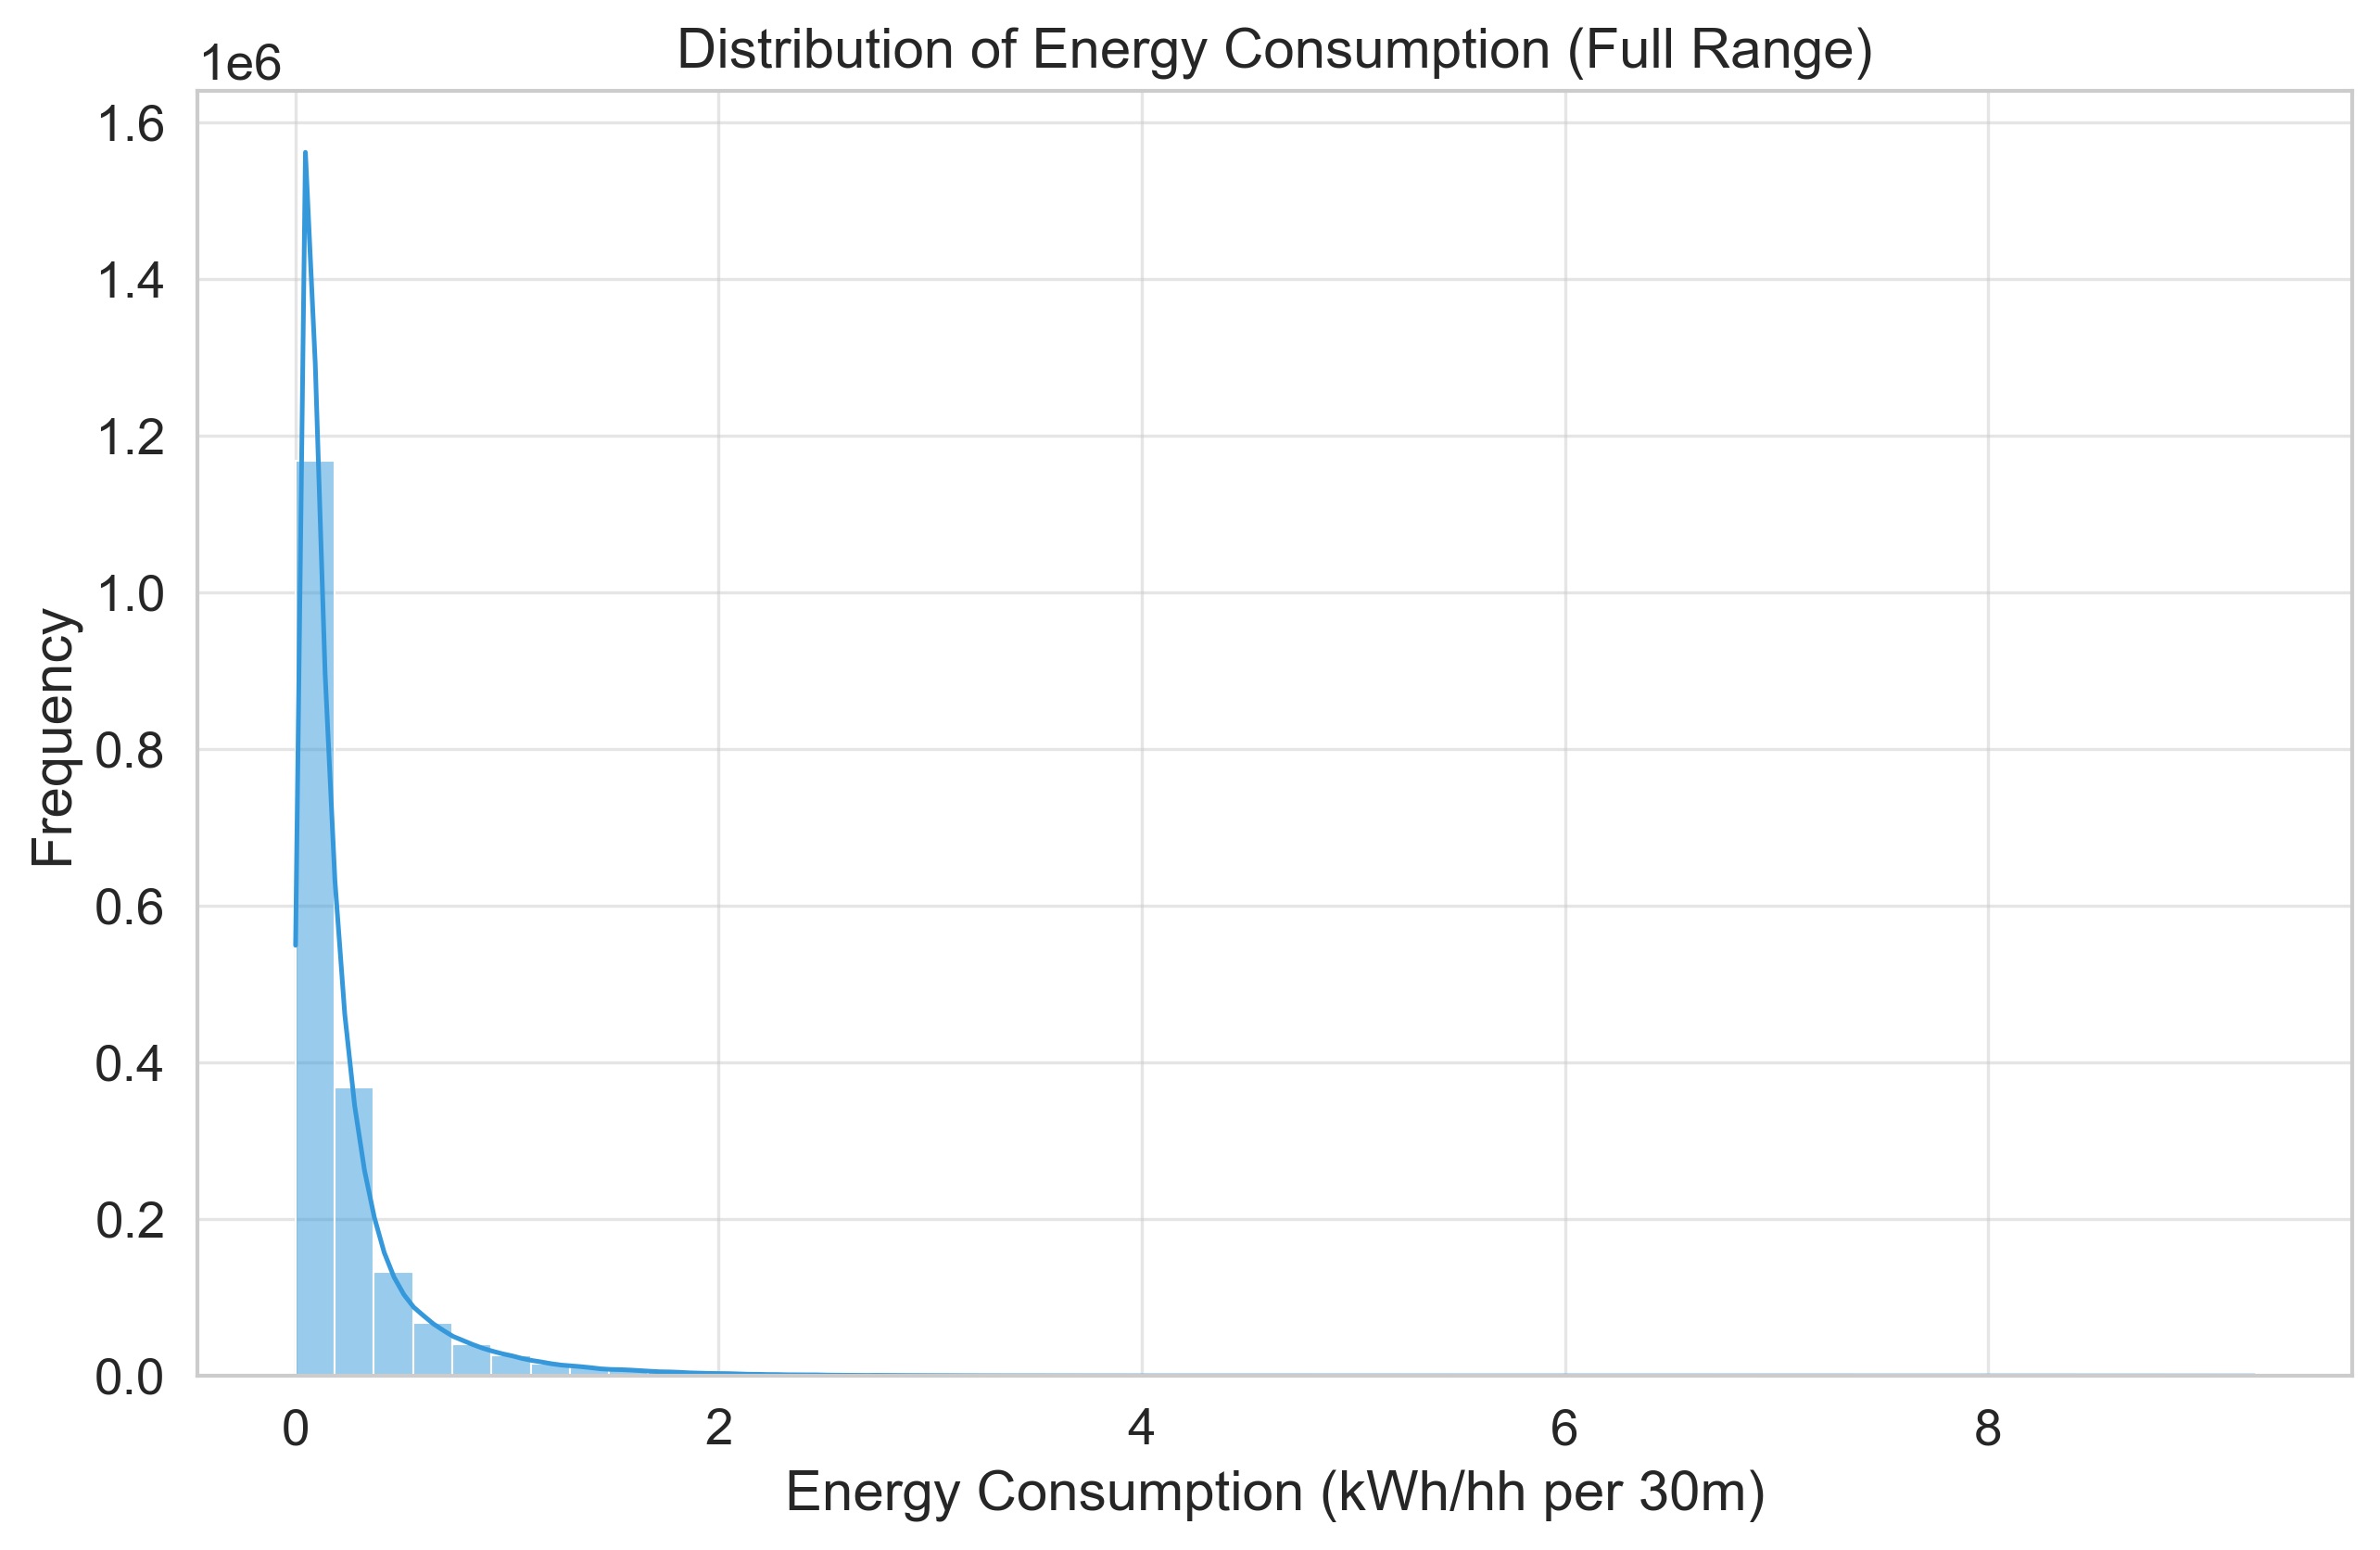
\includegraphics[width=1\textwidth]{figures/distribution_full_range.png}
    \caption{Distribution of raw energy consumption (Scientific Notation).}
    \label{fig:dist_full}
\end{figure}


To better understand the behavior of the majority of the population, Figure \ref{fig:dist_zoomed} provides a focused view of the 0.0 to 1.0 kWh range. This interval is highly significant as it contains approximately 96.5\% of all recorded tuples collected across the entire one-week observation period (336 snapshots) defined in Section~\ref{sec:dataset}. 

\begin{figure}[thp]
    \centering
    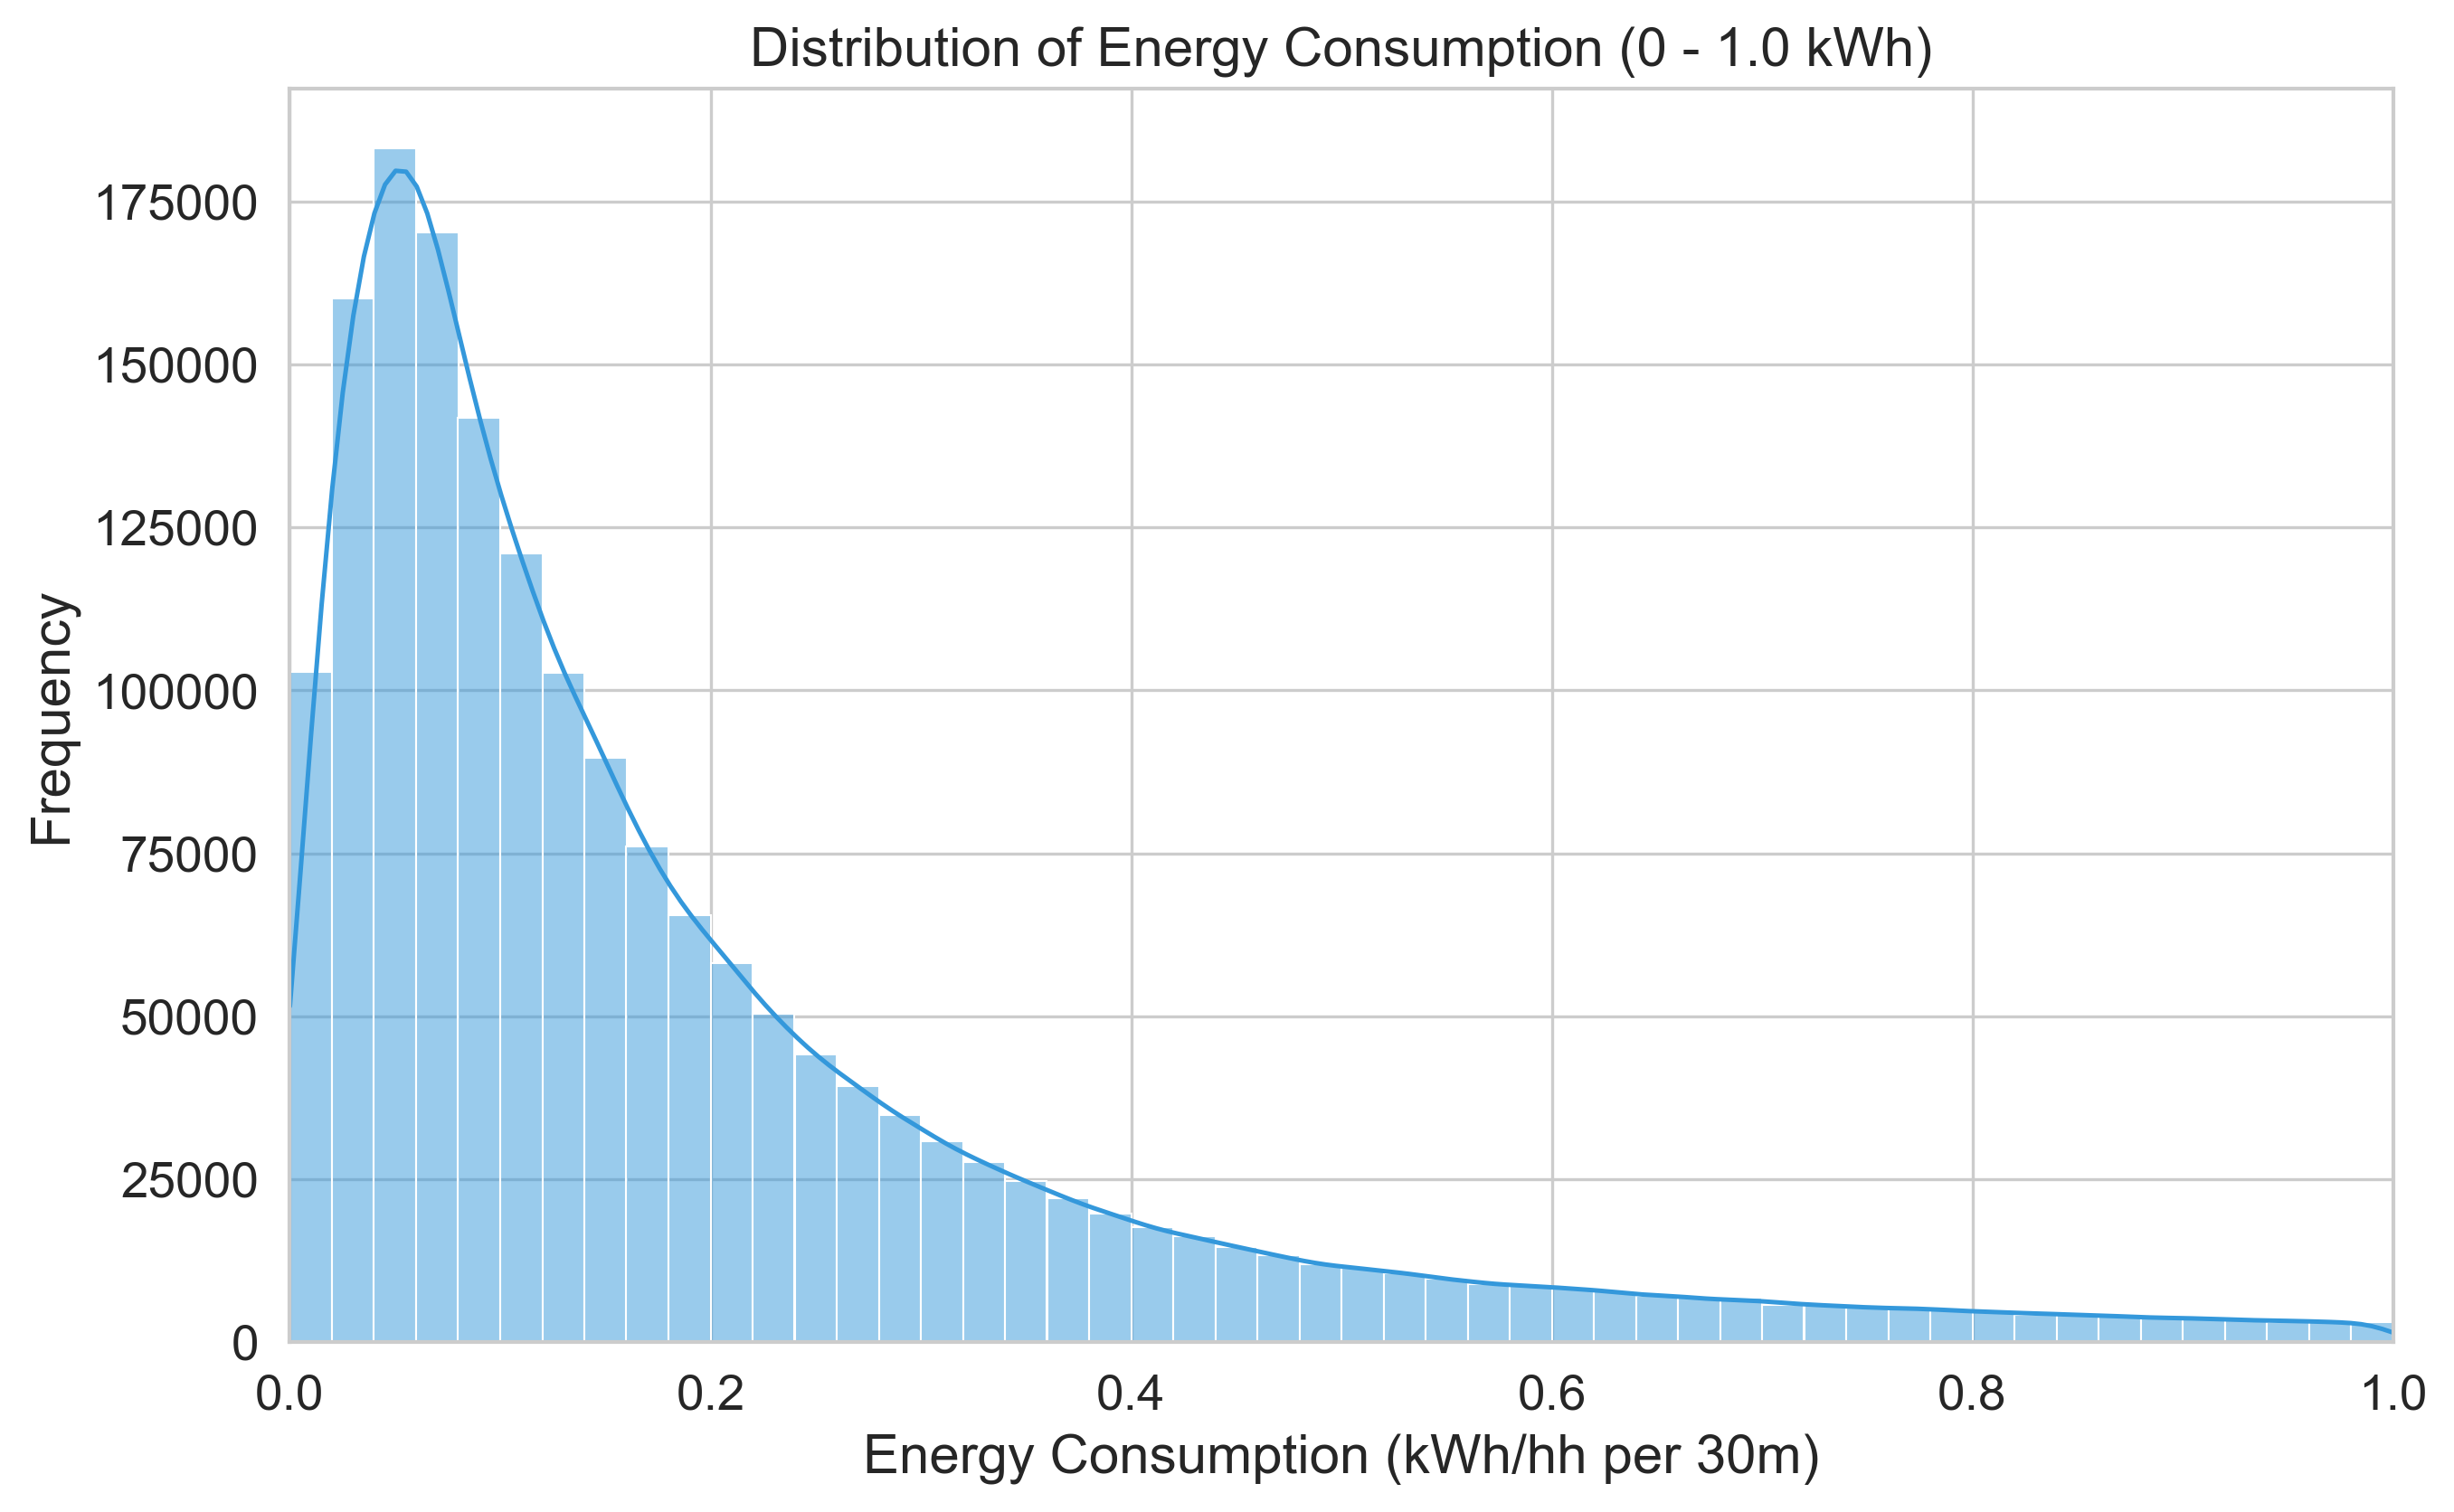
\includegraphics[width=1\textwidth]{figures/distribution_zoomed_to_1kwh.png}
    \caption{Detailed view of the 0-1.0 kWh range, representing 96.5\% of the total population data aggregated over the full one-week duration (Nov 5-11, 2012).}
    \label{fig:dist_zoomed}
\end{figure}

The distribution reveals two primary characteristics:
\begin{enumerate}
    \item \textbf{Low-Load Concentration:} A significant majority of readings are clustered between 0 kWh and 0.2 kWh. In this range, the high density of users suggests a higher probability of satisfying $z$-anonymity thresholds.
    \item \textbf{High-Precision Sparsity:} Despite the apparent density of the low-load range, the data resolution results in a significant number of unique readings. While Figure~\ref{fig:dist_zoomed} shows that a bin at 0.6 kWh contains approximately 10,000 occurrences, this frequency must be interpreted within the temporal and numerical context of the snapshots. 

    First, these 10,000 occurrences are distributed across the entire one-week period, which consists of 336 distinct timestamps (7 days $\times$ 48 half-hour intervals). This results in an average of only $\approx 30$ tuples per bin per snapshot. Second, because each bin (0.02 kWh wide) encompasses 20 distinct measurement values due to the three-decimal-point precision (e.g., 0.600, 0.601, ..., 0.619), the 30 tuples are further fragmented. This results in an average of only \textbf{$\approx 1.5$ occurrences per specific raw value at any given timestamp}. Since $z$-anonymity requires a value to appear at least $z$ times to satisfy the anonymity threshold, the raw high-precision data is effectively "near zero" in terms of publishable frequency. This sparsity at the individual measurement level is the primary driver of the near-total suppression observed in the global \textbf{Baseline performance}, which is further analyzed in Section~\ref{sec:baseline} (Figure~\ref{fig:baseline}).

\end{enumerate}




While the histograms characterize the range of values, energy consumption is inherently temporal. To understand the privacy challenges in a streaming context, we must analyze how user behavior and data sparsity evolve over a daily cycle. Figure \ref{fig:daily_load_sparsity} illustrates the relationship between average consumption and the uniqueness of the data.

As shown in Figure \ref{fig:load_profile}, the dataset exhibits the standard "double-peak" characteristic of residential demand, with a minor morning peak at 08:30 and a major evening peak lasting from 16:00 to 22:00. Figure \ref{fig:sparsity_trend} reveals that the number of unique energy readings follows this consumption curve almost perfectly. 

During the evening peak, the count of unique values rises to approximately 1,250 per snapshot. Within a population of 5,529 users, this indicates that nearly one out of every four users reports a value that is unique to three decimal places during high-activity periods. In contrast, during the early morning hours (02:00--05:00), the number of unique values drops to approximately 580, suggesting a much higher concentration of identical readings during low-load periods. 

The heatmap in Figure \ref{fig:dist_heatmap} confirms that these patterns are consistent across the selected week. While the morning peak shifts slightly during the weekend (Saturday and Sunday), the high entropy associated with evening usage remains a constant characteristic of the dataset.
% \clearpage % images finished before starting the next section 
\begin{figure}[H]
\centering
\begin{subfigure}{0.80\textwidth}
\centering
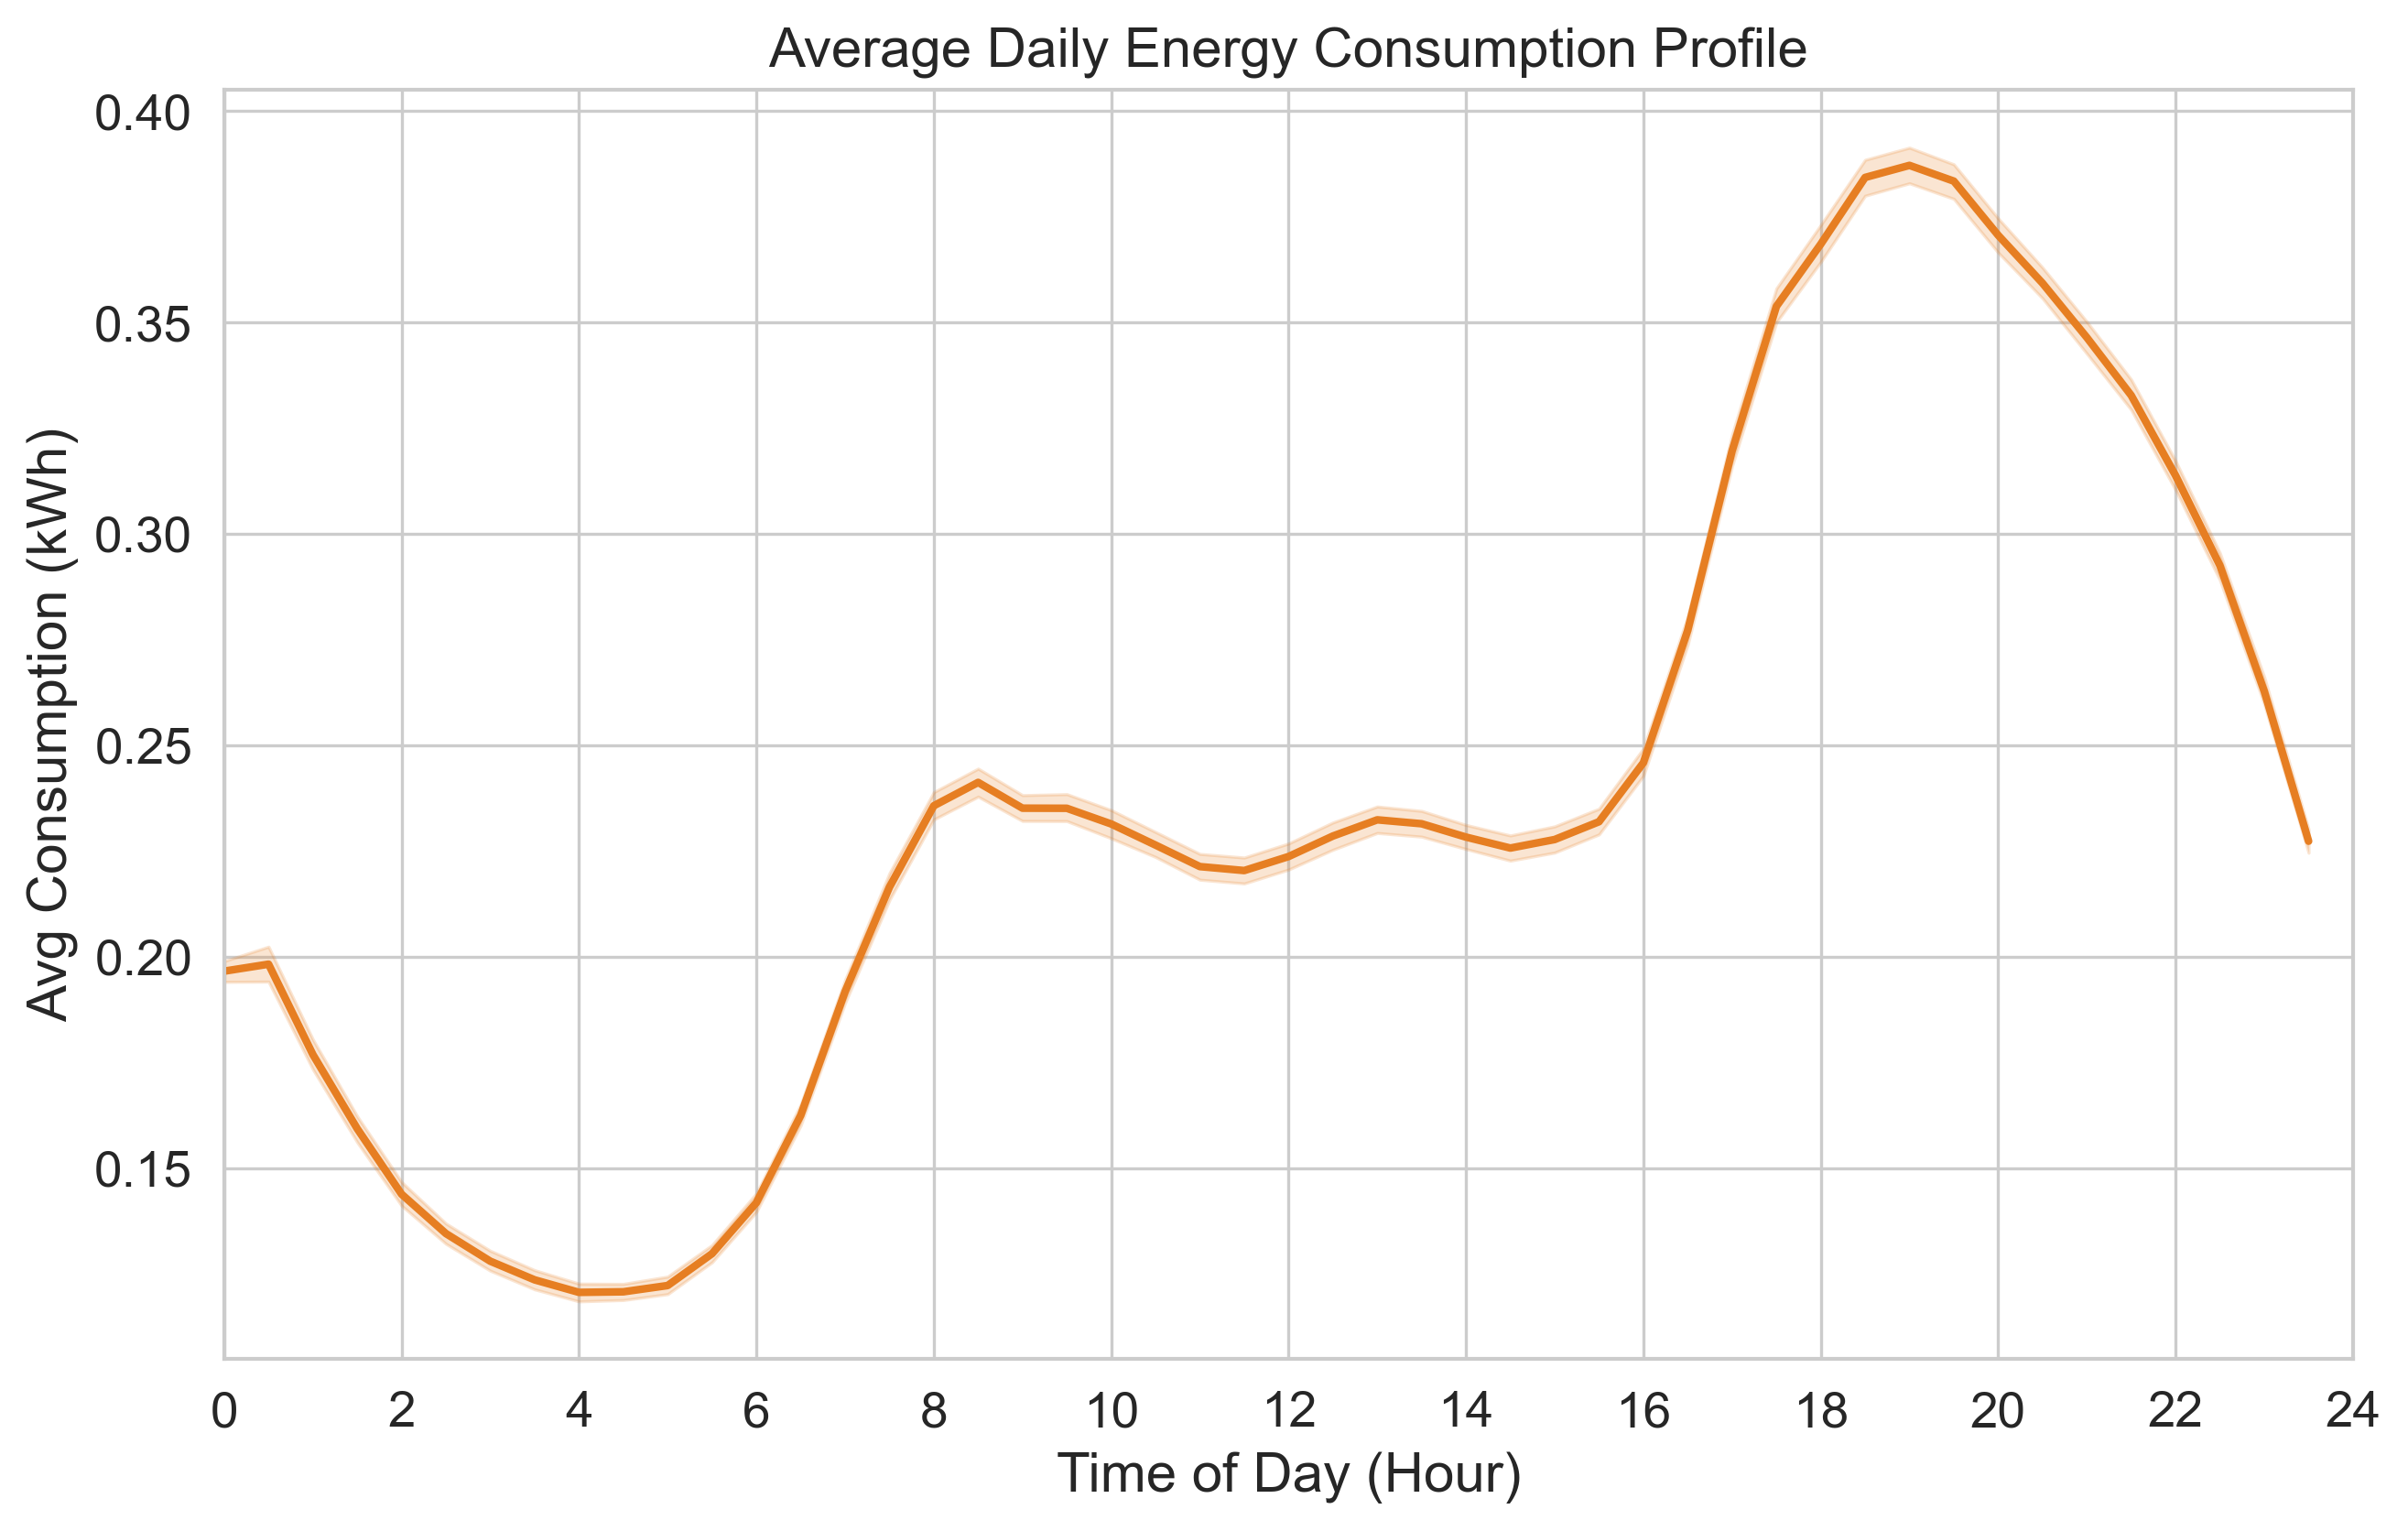
\includegraphics[width=\textwidth]{figures/distribution_daily_profile.png}
\caption{Average Daily Load Profile.}
\label{fig:load_profile}
\end{subfigure}
\hfill
\begin{subfigure}{0.80\textwidth}
\centering
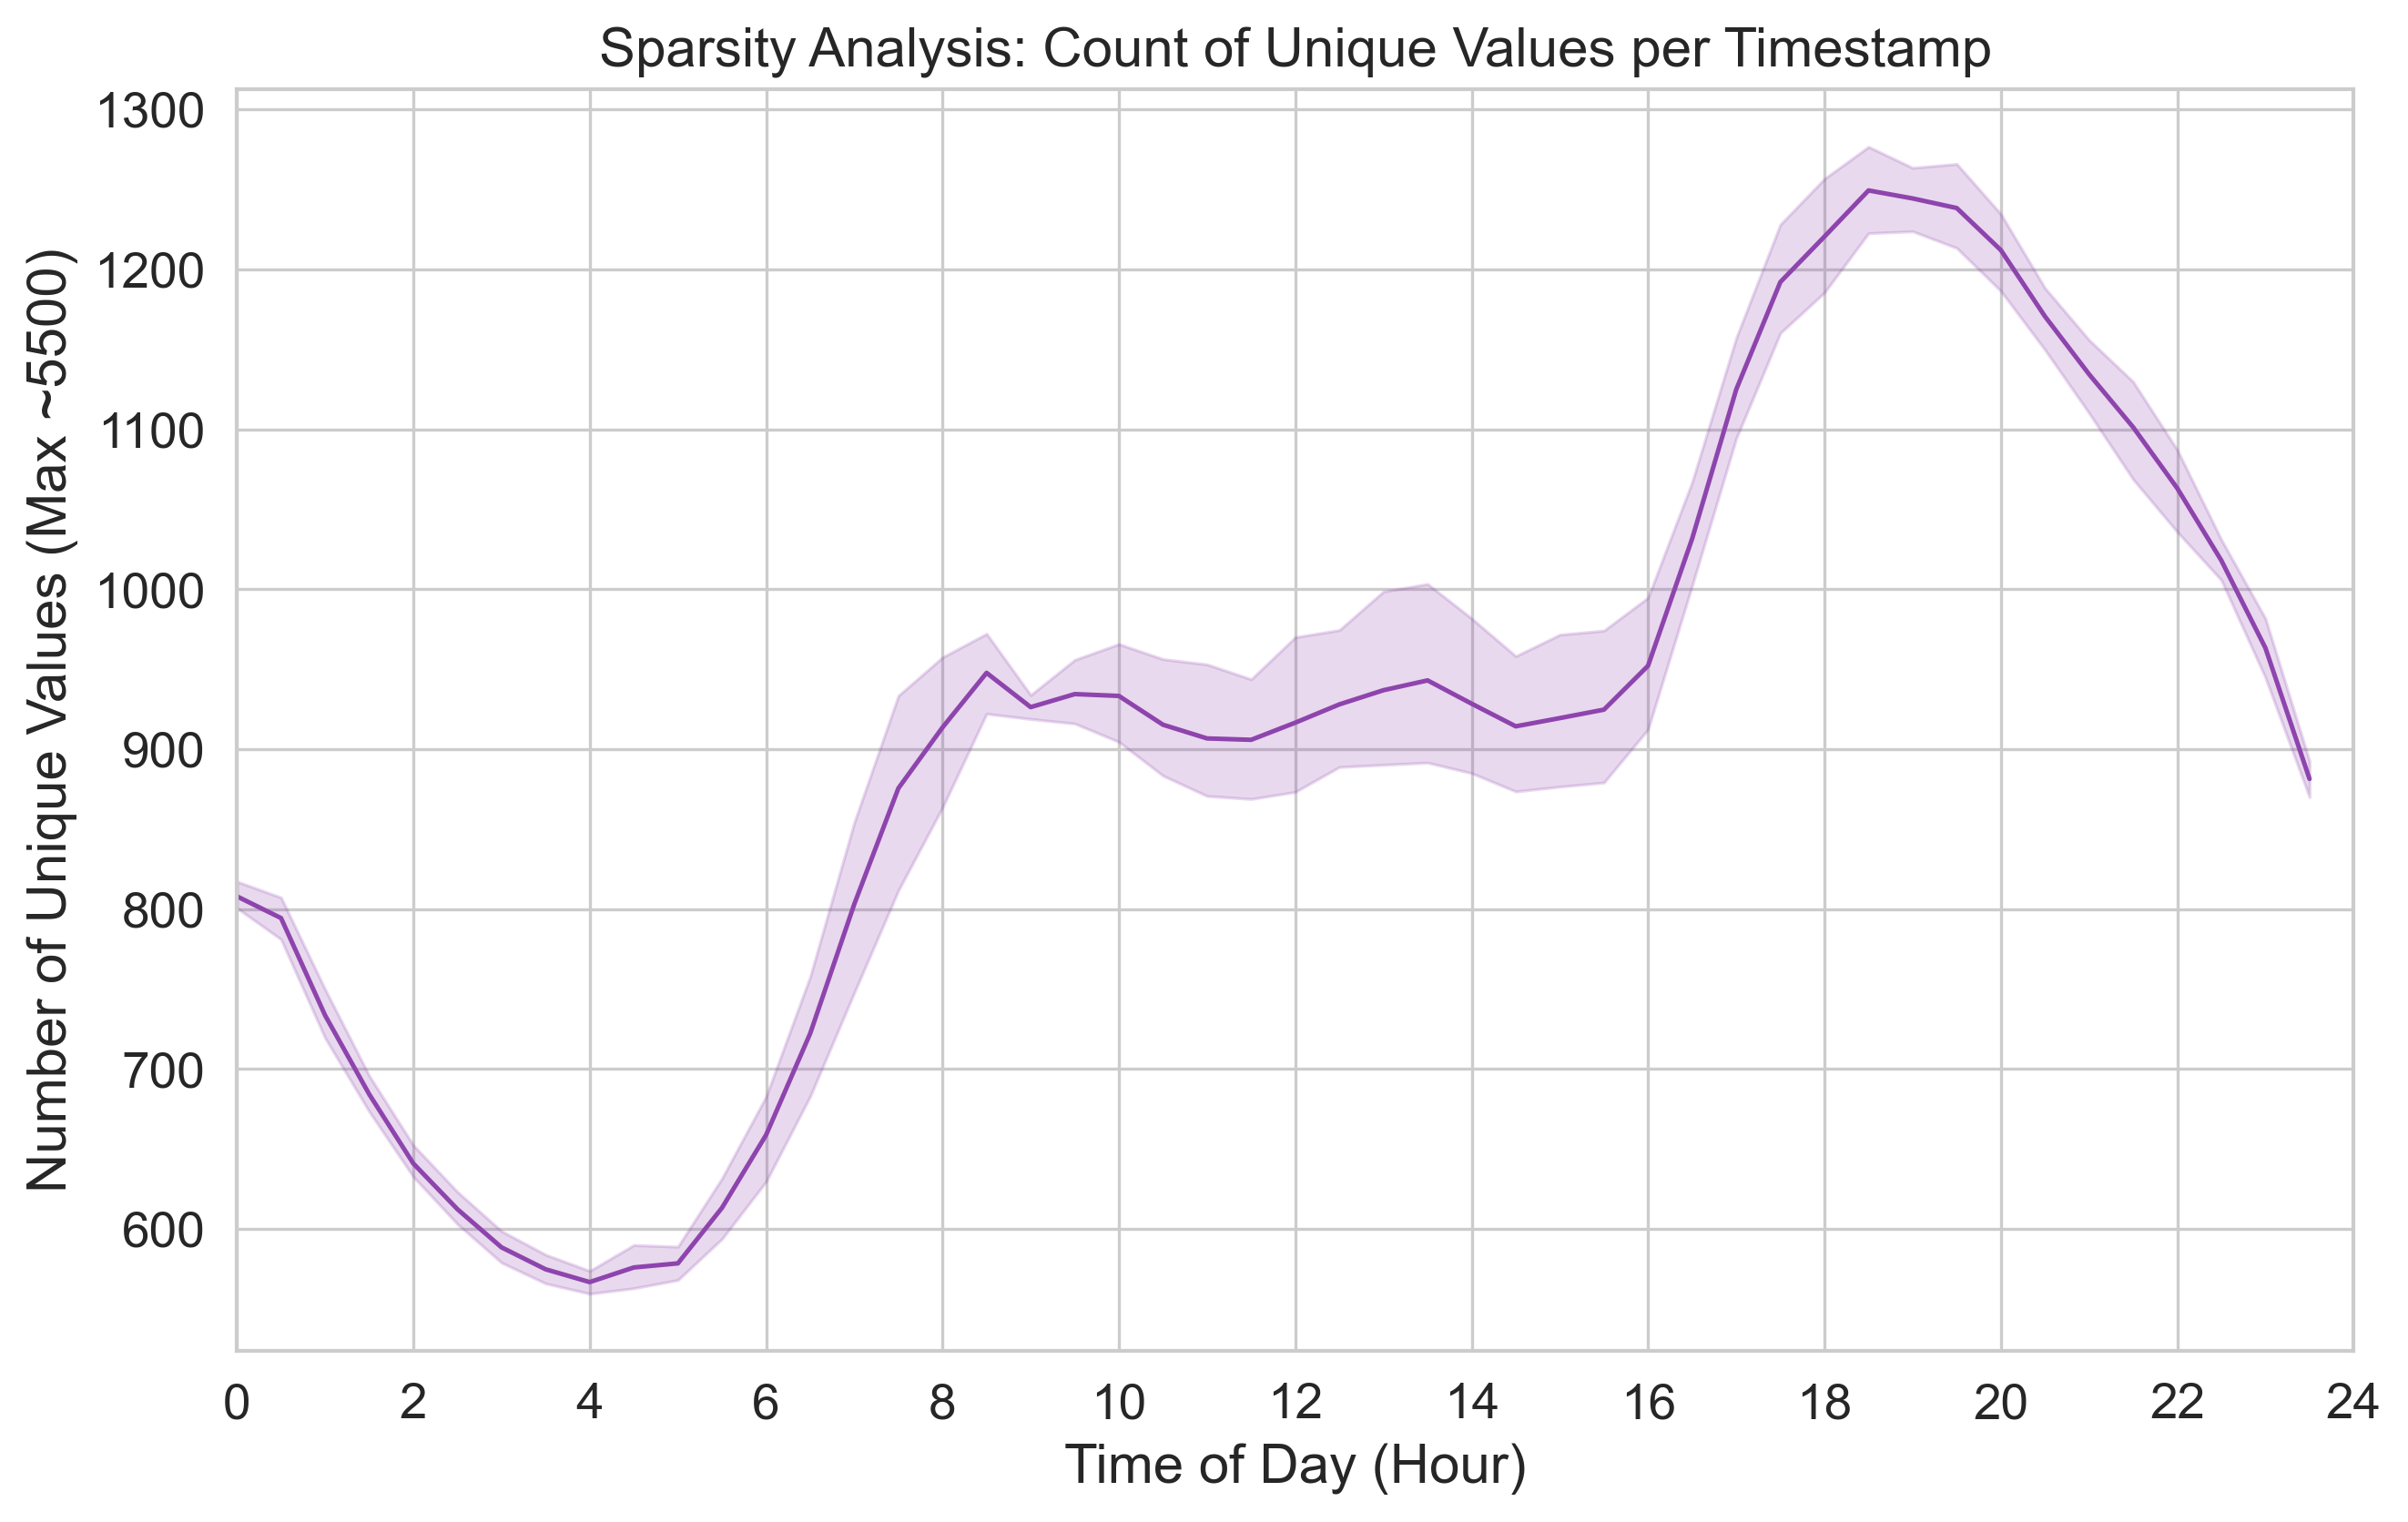
\includegraphics[width=\textwidth]{figures/distribution_sparsity.png}
\caption{Count of Unique Values per Timestamp.}
\label{fig:sparsity_trend}
\end{subfigure}
\hfill
\begin{subfigure}{0.80\textwidth}
\centering
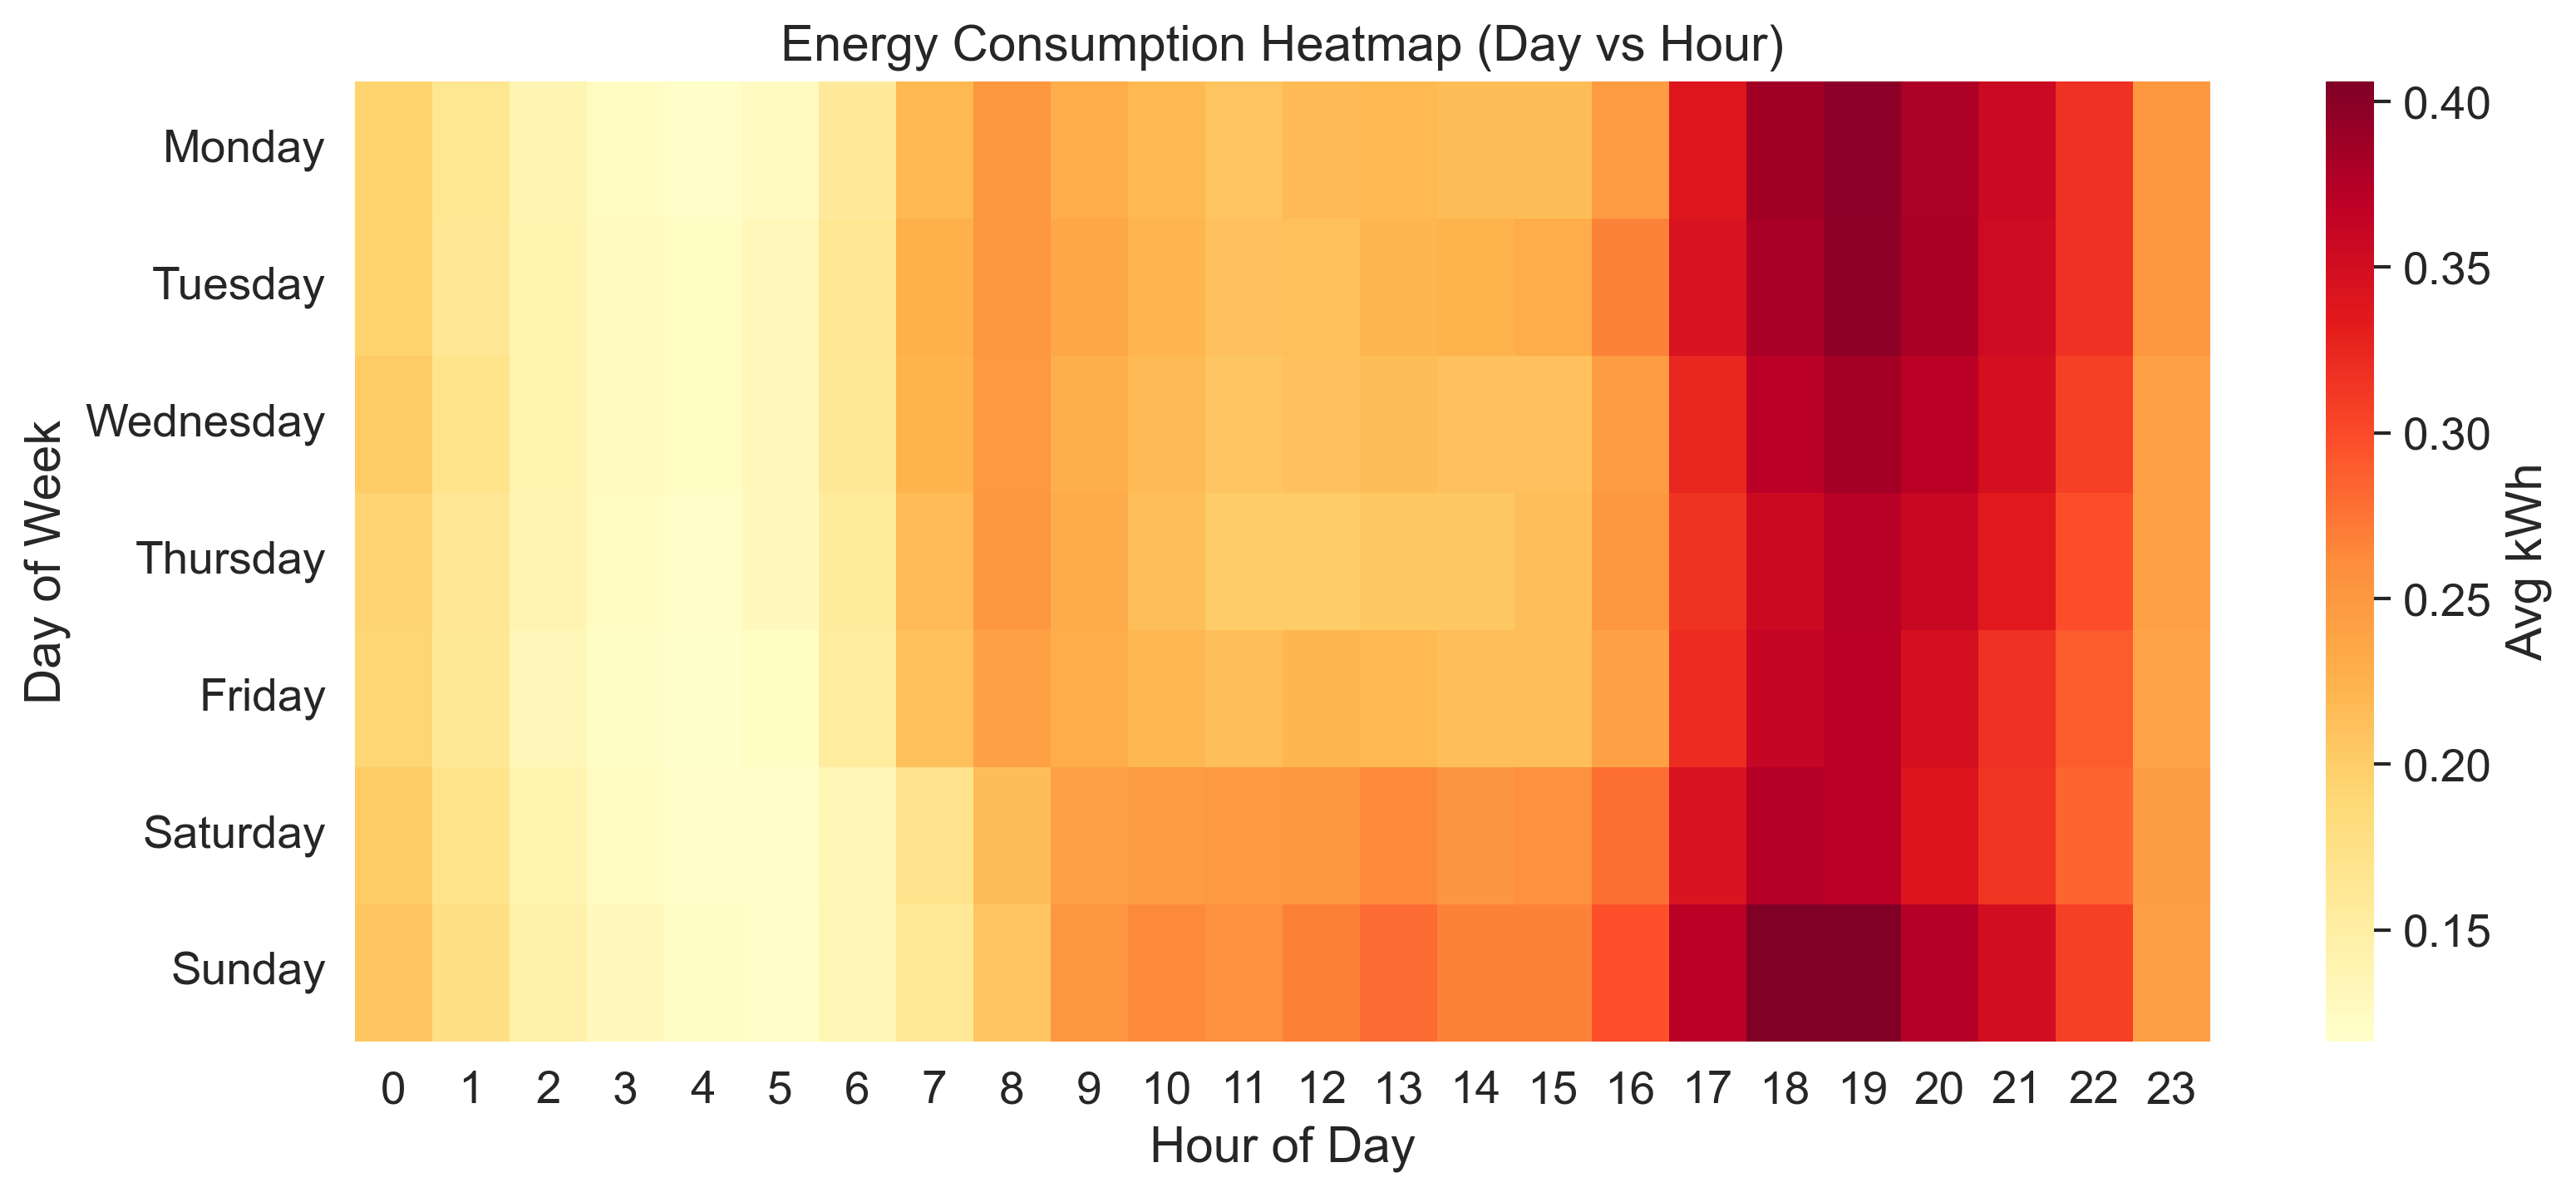
\includegraphics[width=\textwidth]{figures/distribution_heatmap.png}
\caption{Heatmap of energy consumption across the week.}
\label{fig:dist_heatmap}
\end{subfigure}
\caption{Temporal analysis of the dataset over a 24-hour cycle.}
\label{fig:daily_load_sparsity}
\end{figure}


% As shown in Figure \ref{fig:load_profile}, the dataset exhibits the standard "double-peak" characteristic of residential demand, with a minor morning peak at 08:30 and a major evening peak lasting from 16:00 to 22:00. Figure \ref{fig:sparsity_trend} reveals that the number of unique energy readings follows this consumption curve almost perfectly. 

% During the evening peak, the count of unique values rises to approximately 1,250 per snapshot. Within a population of 5,529 users, this indicates that nearly one out of every four users reports a value that is unique to three decimal places during high-activity periods. In contrast, during the early morning hours (02:00--05:00), the number of unique values drops to approximately 580, suggesting a much higher concentration of identical readings during low-load periods. 

% The heatmap in Figure \ref{fig:dist_heatmap} confirms that these patterns are consistent across the selected week. While the morning peak shifts slightly during the weekend (Saturday and Sunday), the high entropy associated with evening usage remains a constant characteristic of the dataset.

% \begin{figure}[H]
% \centering
% 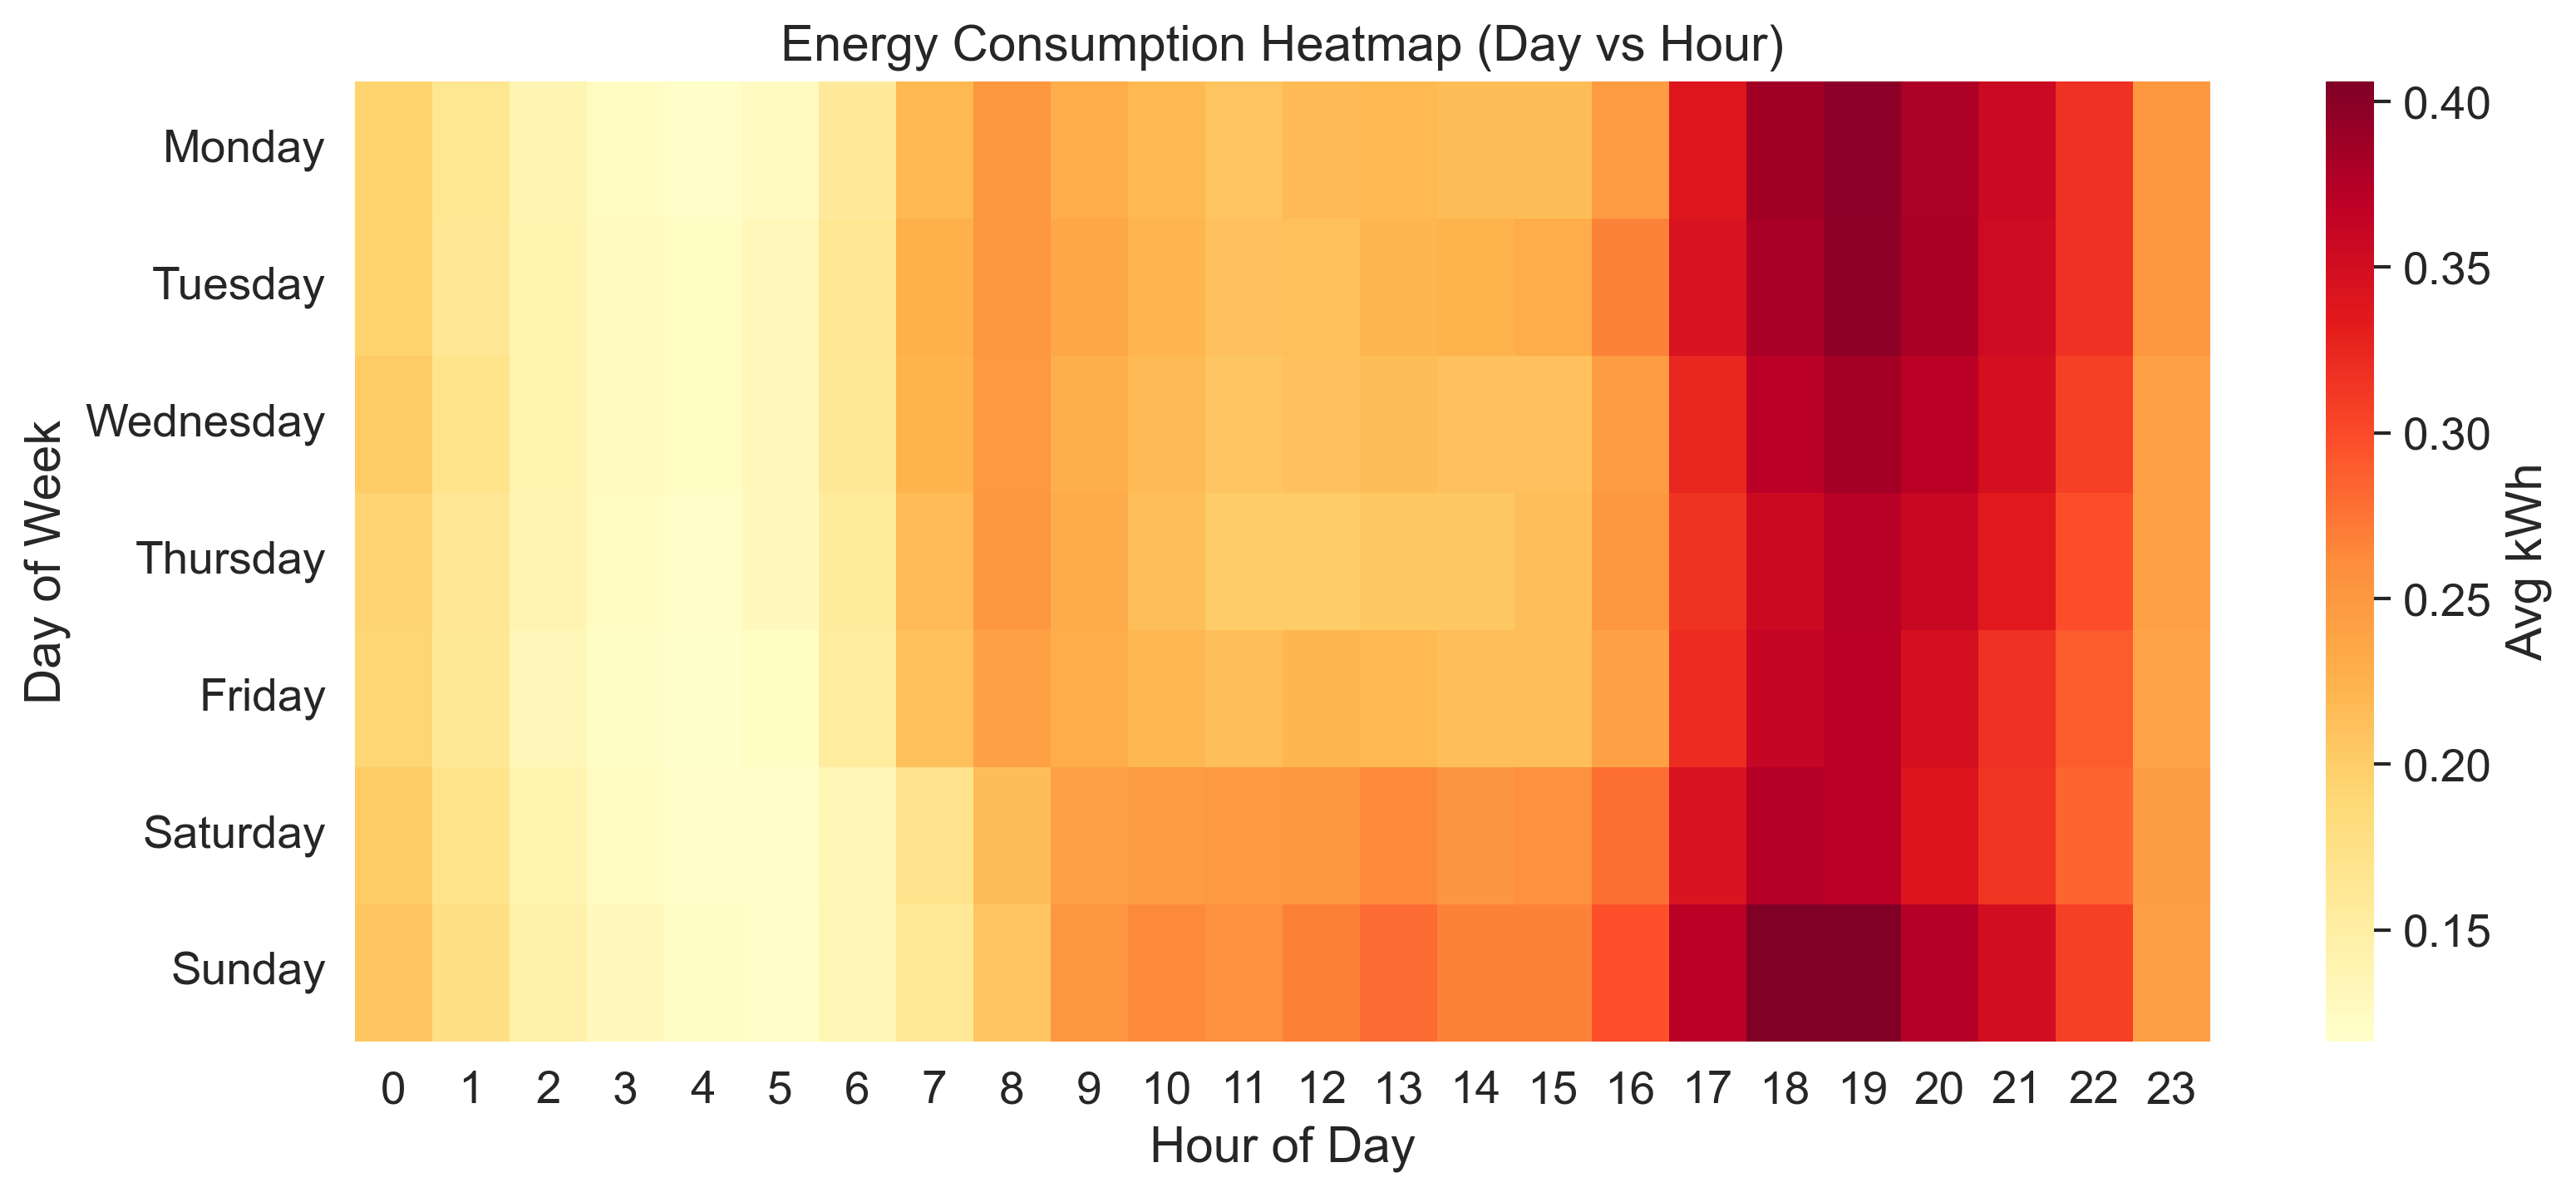
\includegraphics[width=0.9\textwidth]{figures/distribution_heatmap.png}
% \caption{Heatmap of energy consumption across the week.}
% \label{fig:dist_heatmap}
% \end{figure}

\section{Baseline Performance (Cloud-Only)}
\label{sec:baseline}
The Baseline scenario represents the centralized approach where raw data is transmitted directly to the Cloud before the privacy check is applied. This serves as the control group for the experiments.

Figure \ref{fig:baseline} depicts the Publication Ratio as a function of the privacy threshold $z$. The results indicate a rapid degradation of data availability as the privacy requirement increases.

\begin{figure}[H]
    \centering
    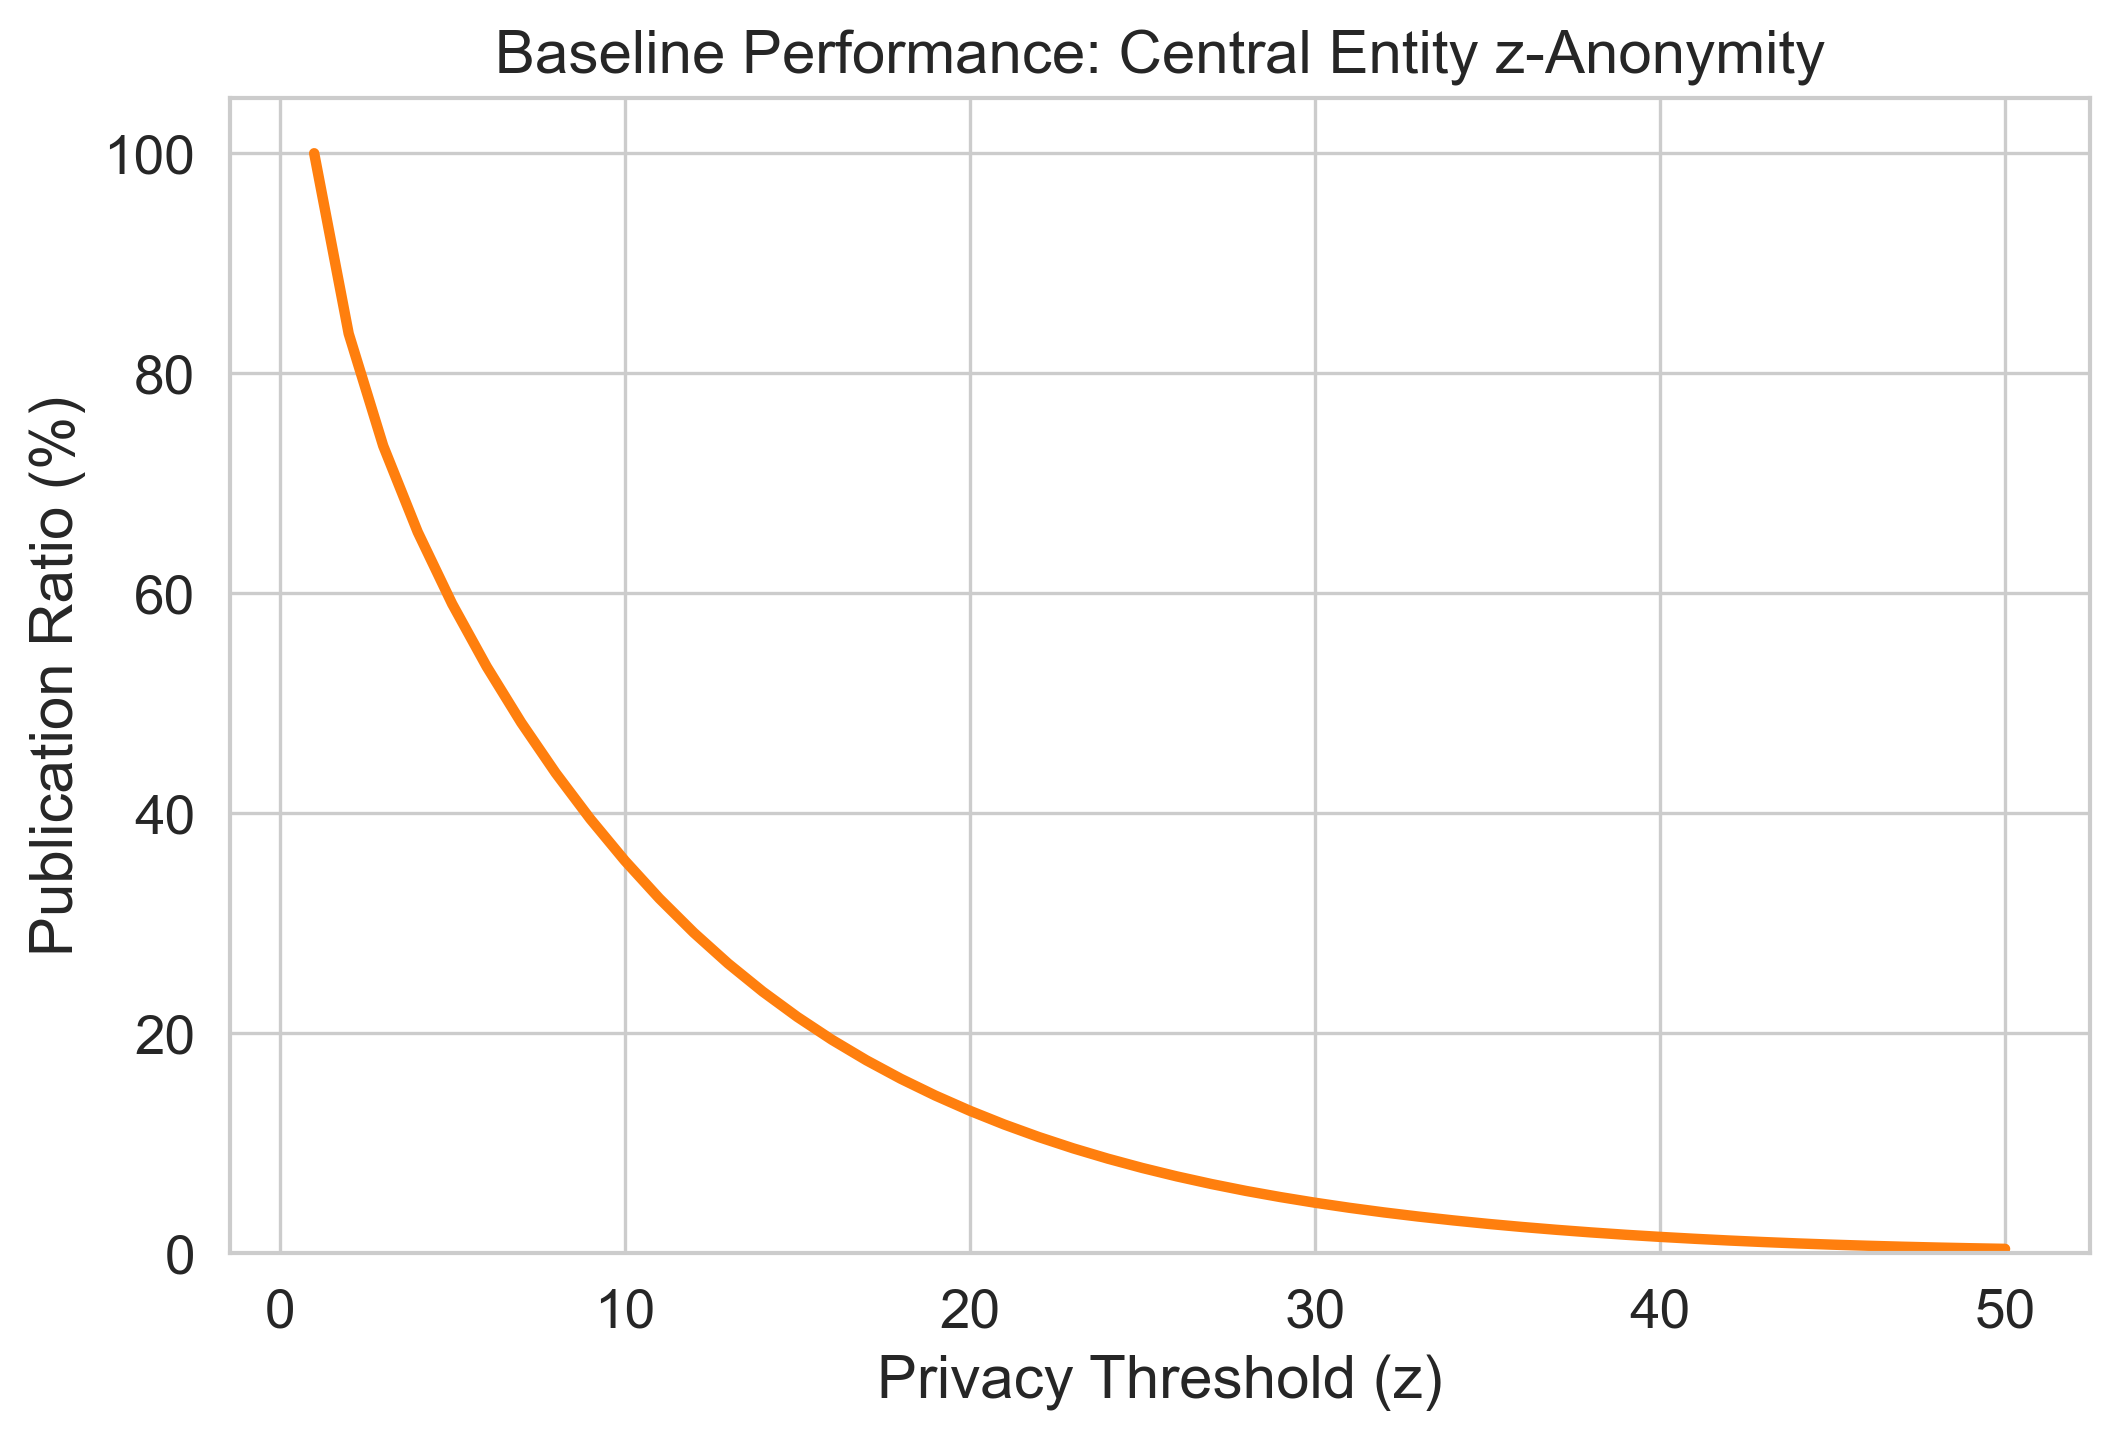
\includegraphics[width=0.82\textwidth]{figures/results_baseline.png}
    \caption{Baseline Performance: Publication Ratio vs. $z$.}
    \label{fig:baseline}
\end{figure}

Consistent with the sparsity observed in the data distribution analysis, the system struggles to maintain availability:
\begin{itemize}
    \item \textbf{At $z=2$:} The system publishes 83.6\% of the tuples.
    \item \textbf{At $z=10$:} The publication ratio drops to approximately 35.7\%.
    \item \textbf{At $z=50$:} The publication ratio falls below 0.4\%.
\end{itemize}

Given the total population of 5,529 households, finding at least two matching consumption readings at a single timestamp is statistically probable, especially within the low-load ranges identified in Section~\ref{sec:datadistribution}. This explains the relatively high data availability at $z=2$. However, as the threshold increases toward $z=50$, the high resolution of the raw data (three decimal places) makes it statistically improbable that 50 households will report the identical consumption value simultaneously. Consequently, the probability of satisfying a strict threshold like $z=50$ is near zero, leading to the near-total suppression of the dataset.


\section{Impact of Data Generalization}

The second experimental scenario evaluates the effectiveness of reducing numerical precision at the Edge Layer to improve the global publication ratio. The objective of this approach is to address the significant number of unique readings identified in the baseline analysis. By rounding energy consumption readings, we mathematically increase the probability that multiple users will report identical values within the same 30-minute snapshot, thereby facilitating the formation of the required "crowd" of size $z$.


Figure \ref{fig:results_gen_ratio} illustrates the publication ratio for three levels of precision ($p \in \{0, 1, 2\}$) compared against the high-precision Baseline ($p=3$).
The results demonstrate a dramatic improvement in data availability as data resolution is reduced:
\begin{itemize}
    \item \textbf{Precision 0 (Integer):} Provides the highest data availability, maintaining a publication ratio above 97\% across the entire tested range, including the strictest threshold of $z=50$.
    \item \textbf{Precision 1 (0.1 kWh):} Maintains a high publication ratio, staying above 87\% even at $z=50$, which indicates that most tuples successfully satisfy the privacy constraint at this resolution.
    \item \textbf{Precision 2 (0.01 kWh):} Shows a clear improvement over the high-precision Baseline but remains sensitive to the threshold; the publication ratio drops to 52\% at $z=50$.
\end{itemize}

\begin{figure}[H]
\centering
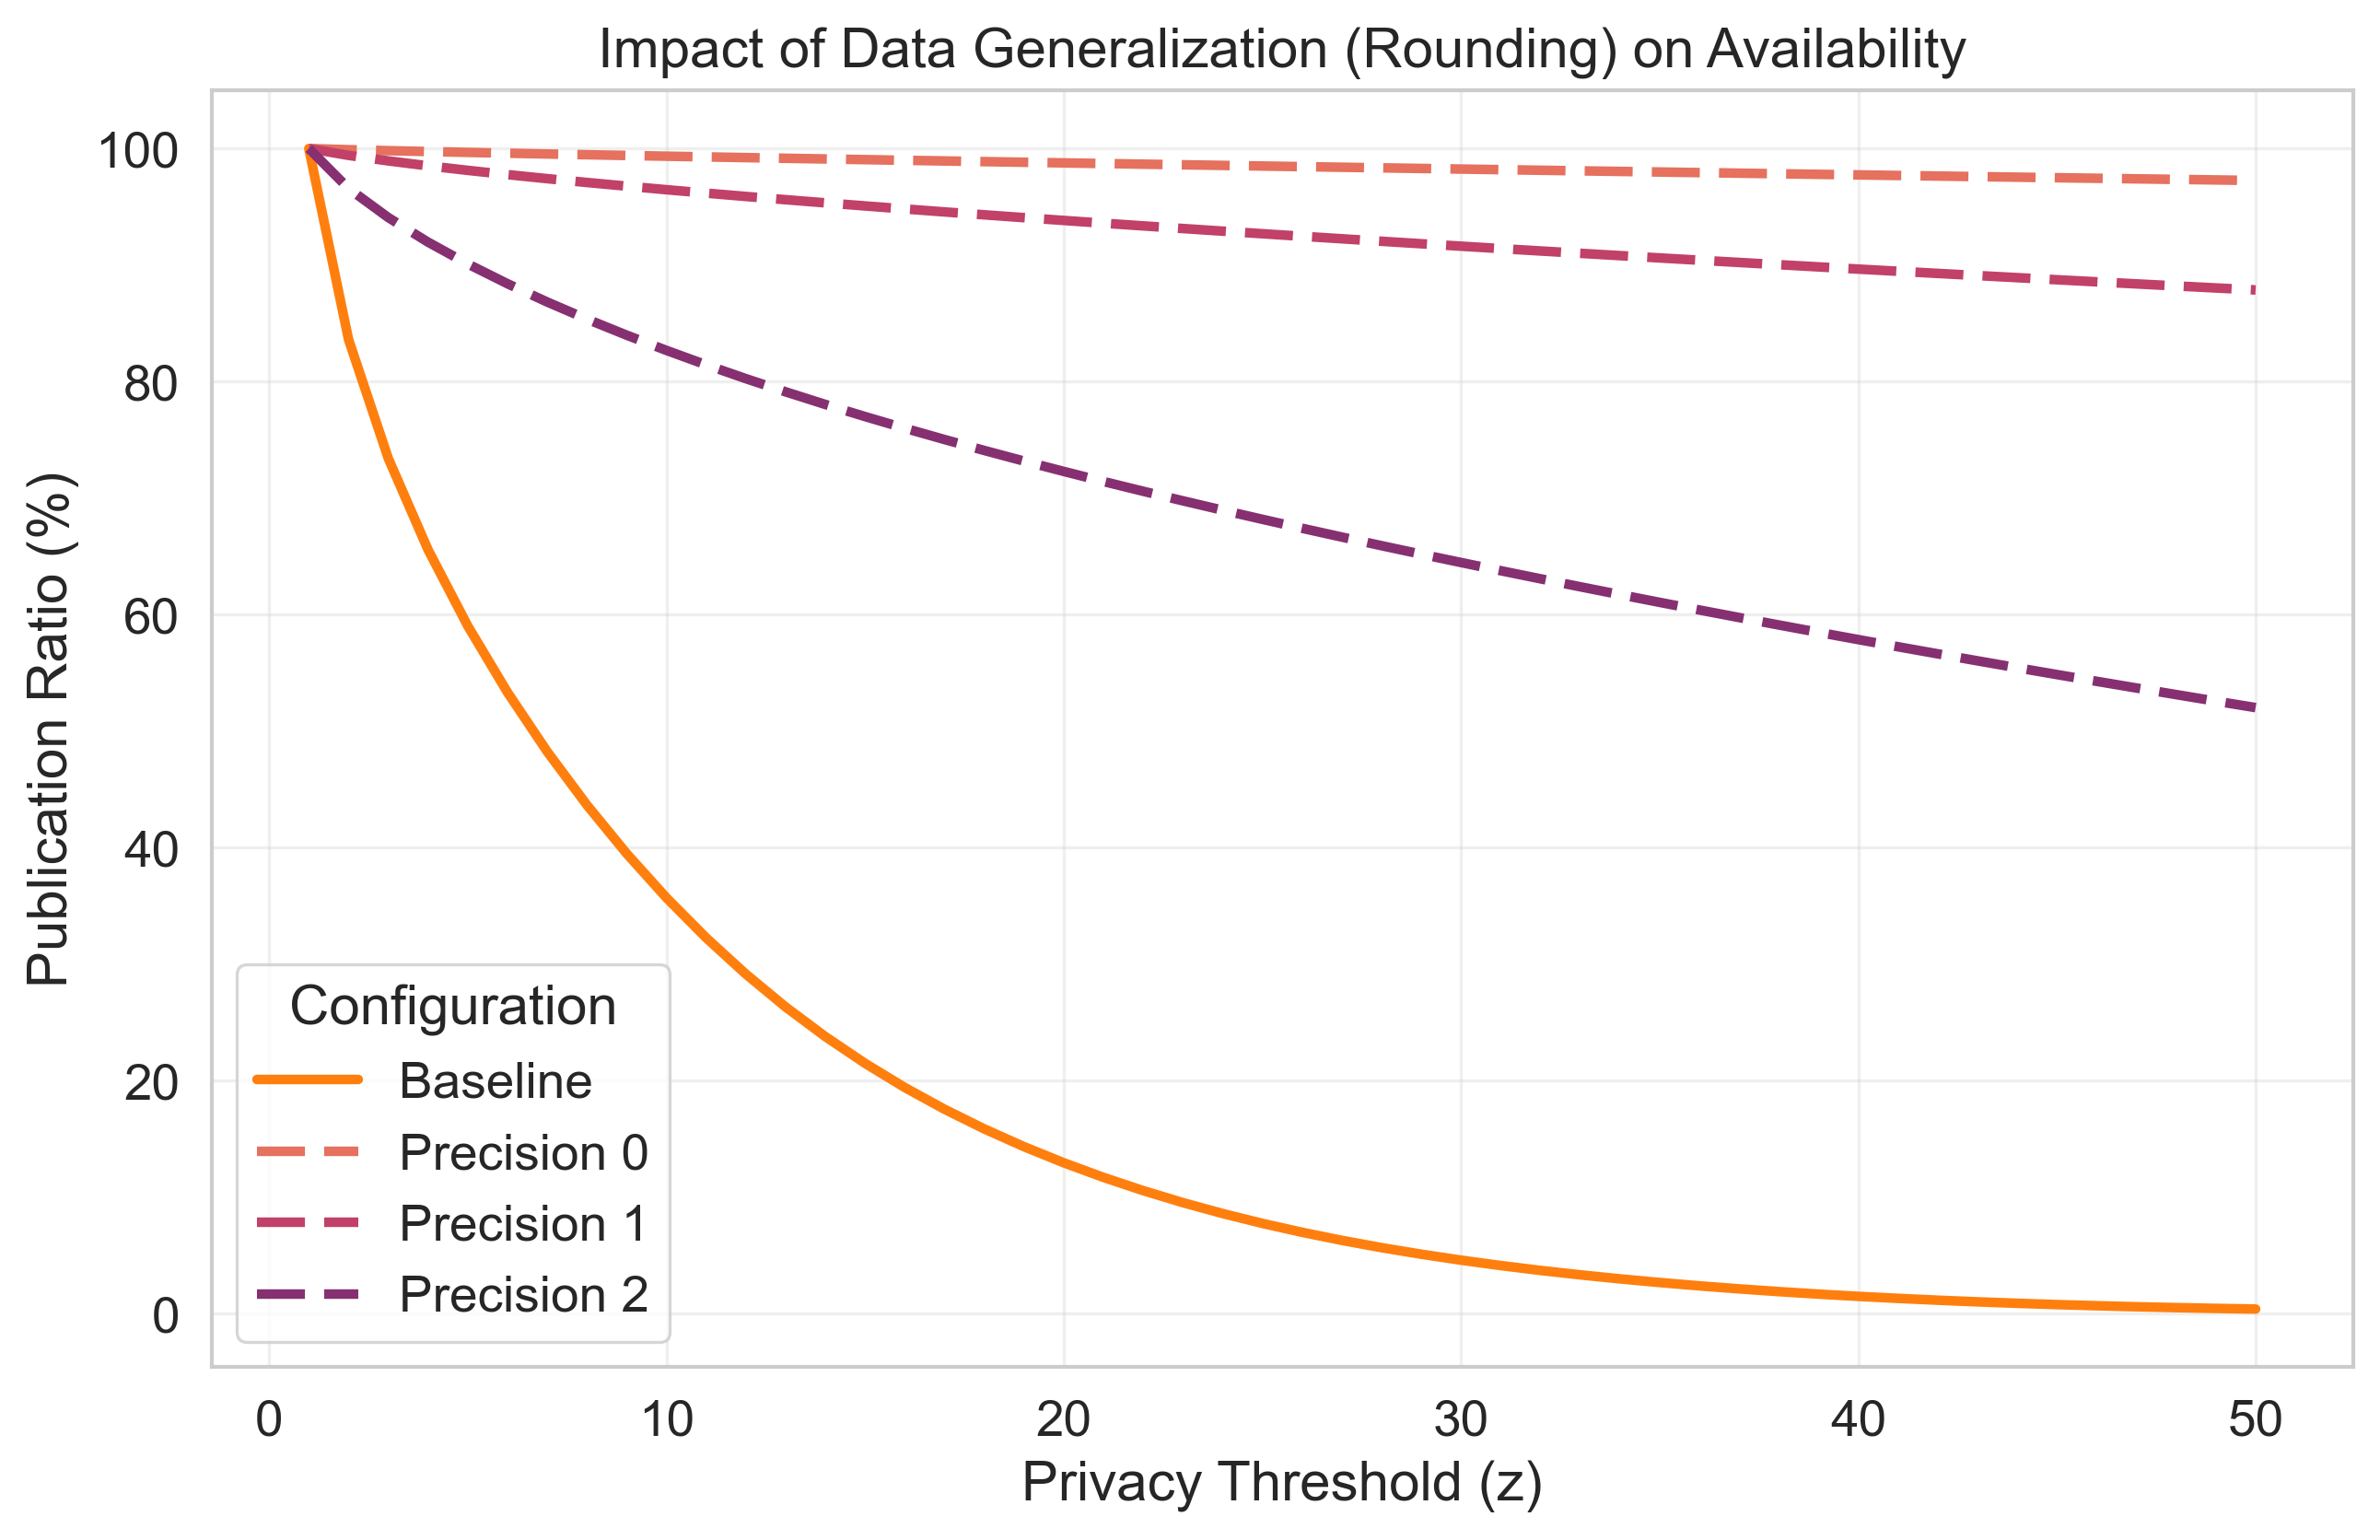
\includegraphics[width=0.8\textwidth]{figures/results_generalization_ratio.png}
\caption{Impact of Data Generalization on Publication Ratio. Lower precision leads to significantly higher data availability.}
\label{fig:results_gen_ratio}
\end{figure}




While reducing precision successfully prevents data suppression, it introduces a permanent loss of information. This cost is first quantified using the $\text{NCP}_{\text{std}}$ metric~\cite{UtilityBasedAnonymizationNCP}, which normalizes the rounding error against the global data range [0, 9.26 kWh].

\begin{figure}[t]
\centering
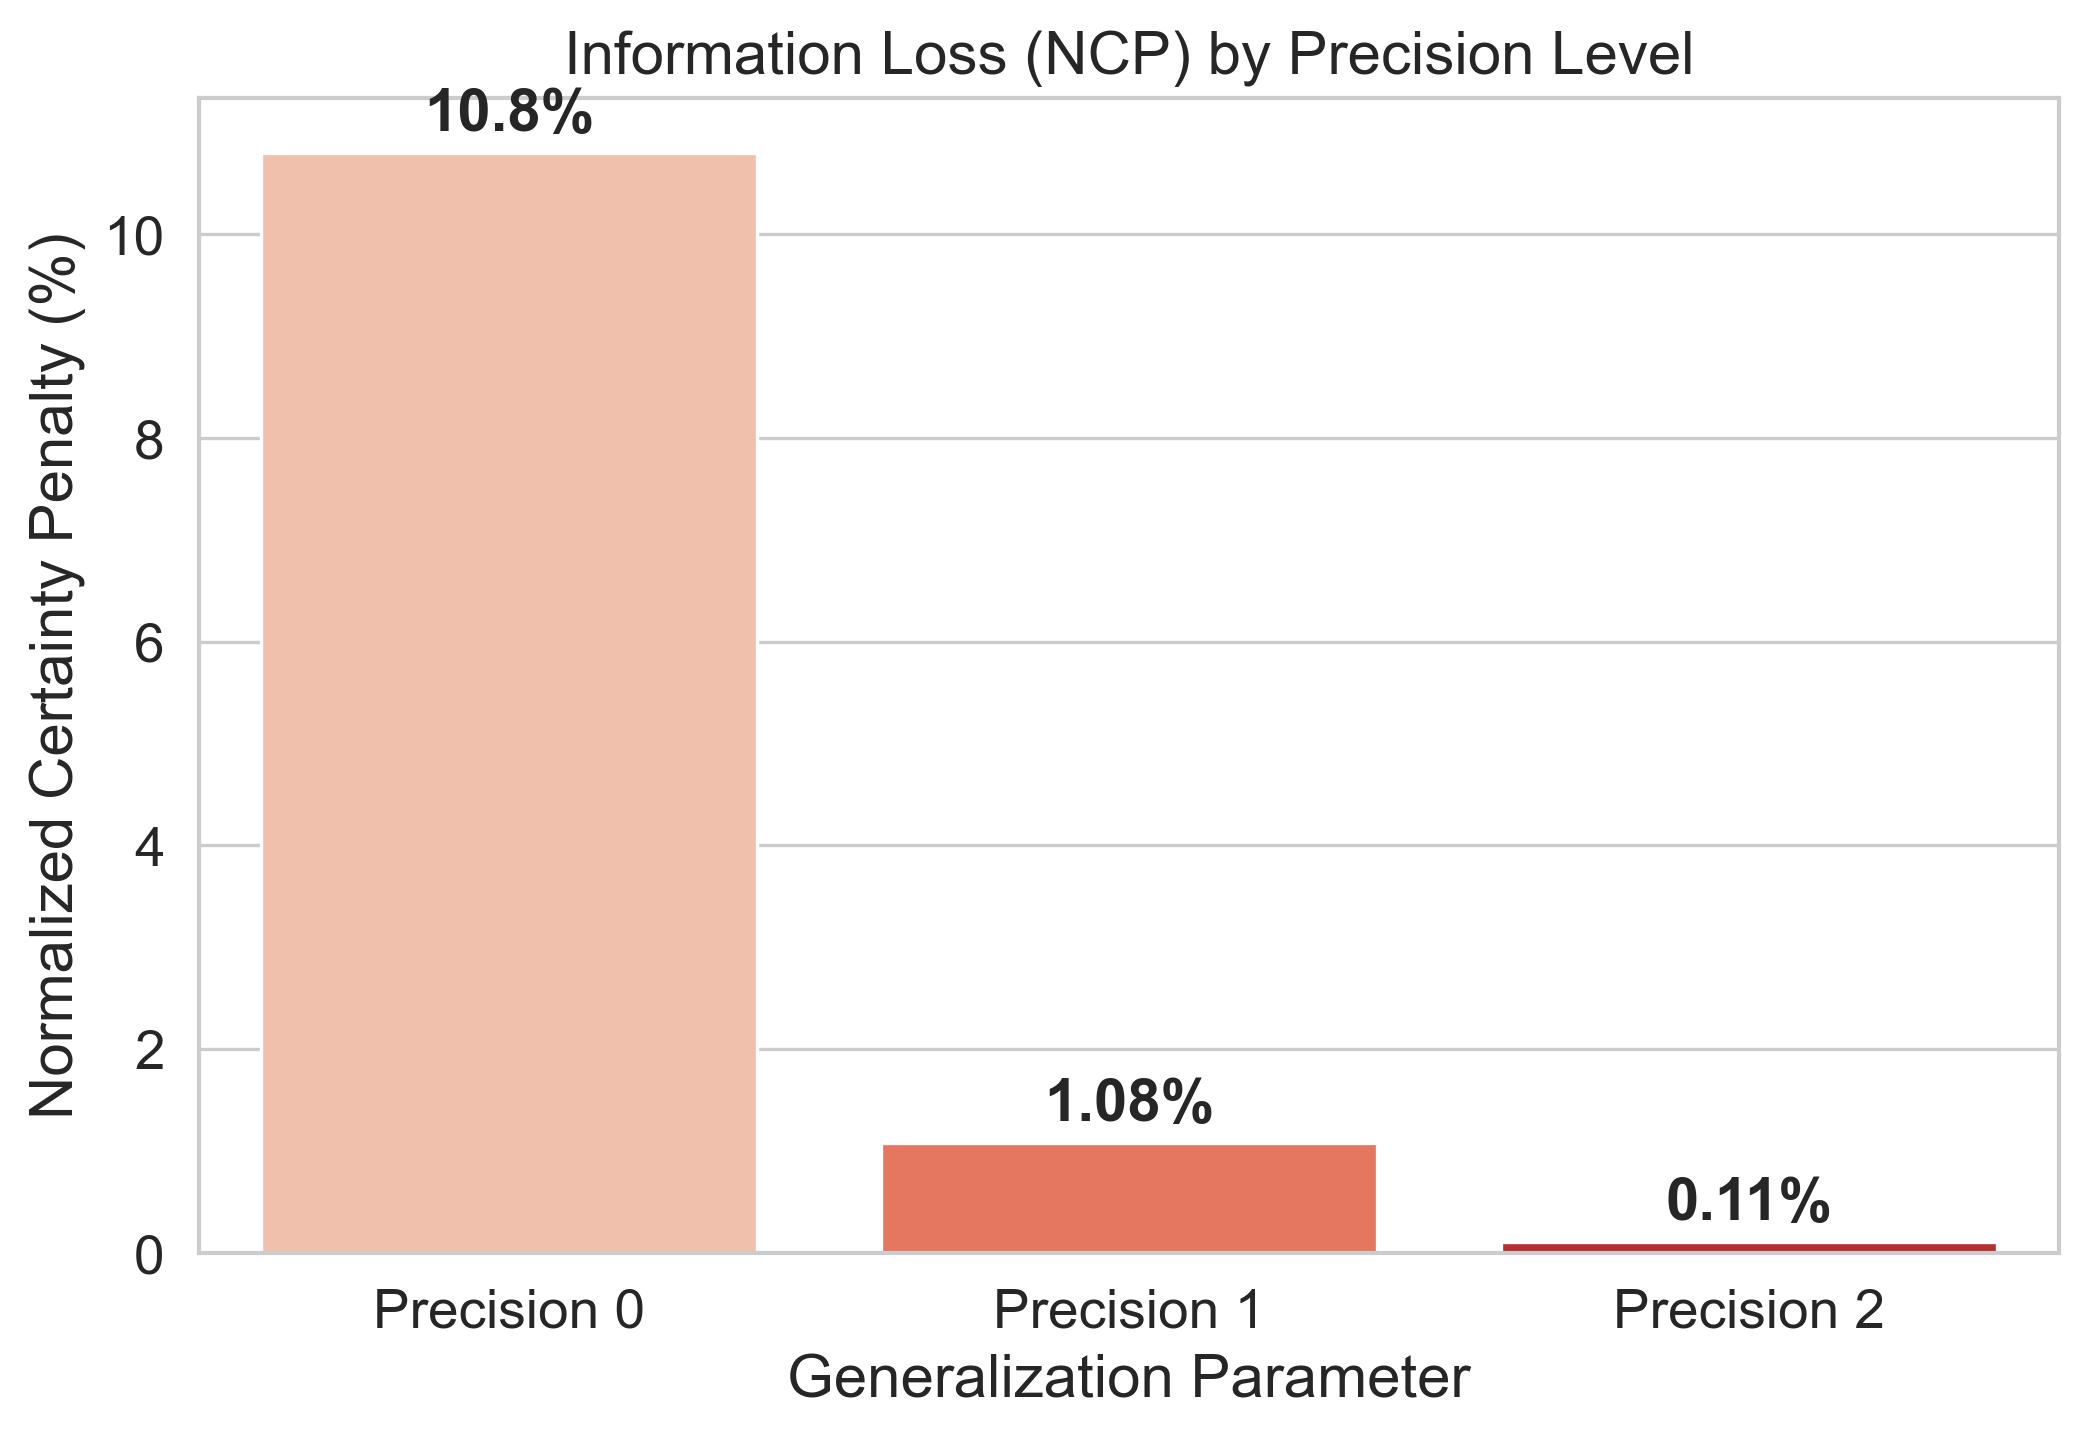
\includegraphics[width=0.77\textwidth]{figures/results_generalization_ncp.png}
\caption{Standard Normalized Certainty Penalty (NCP) for each precision level. The low values suggest a high preservation of global utility.}
\label{fig:results_ncp_std}
\end{figure}

As shown in Figure \ref{fig:results_ncp_std}, the $\text{NCP}_{\text{std}}$ indicates a loss of only 10.8\% for Precision 0 and a negligible 1.1\% for Precision 1. However, these results are skewed by the wide global range caused by outliers, which masks the actual impact of rounding on typical households. To provide a more critical assessment of the utility remaining for the typical user, we contrast these results with the ($\text{NCP}_{\text{eff}}$) defined in Section~\ref{sec:evaluation_metrics}.

\begin{figure}[H]
\centering
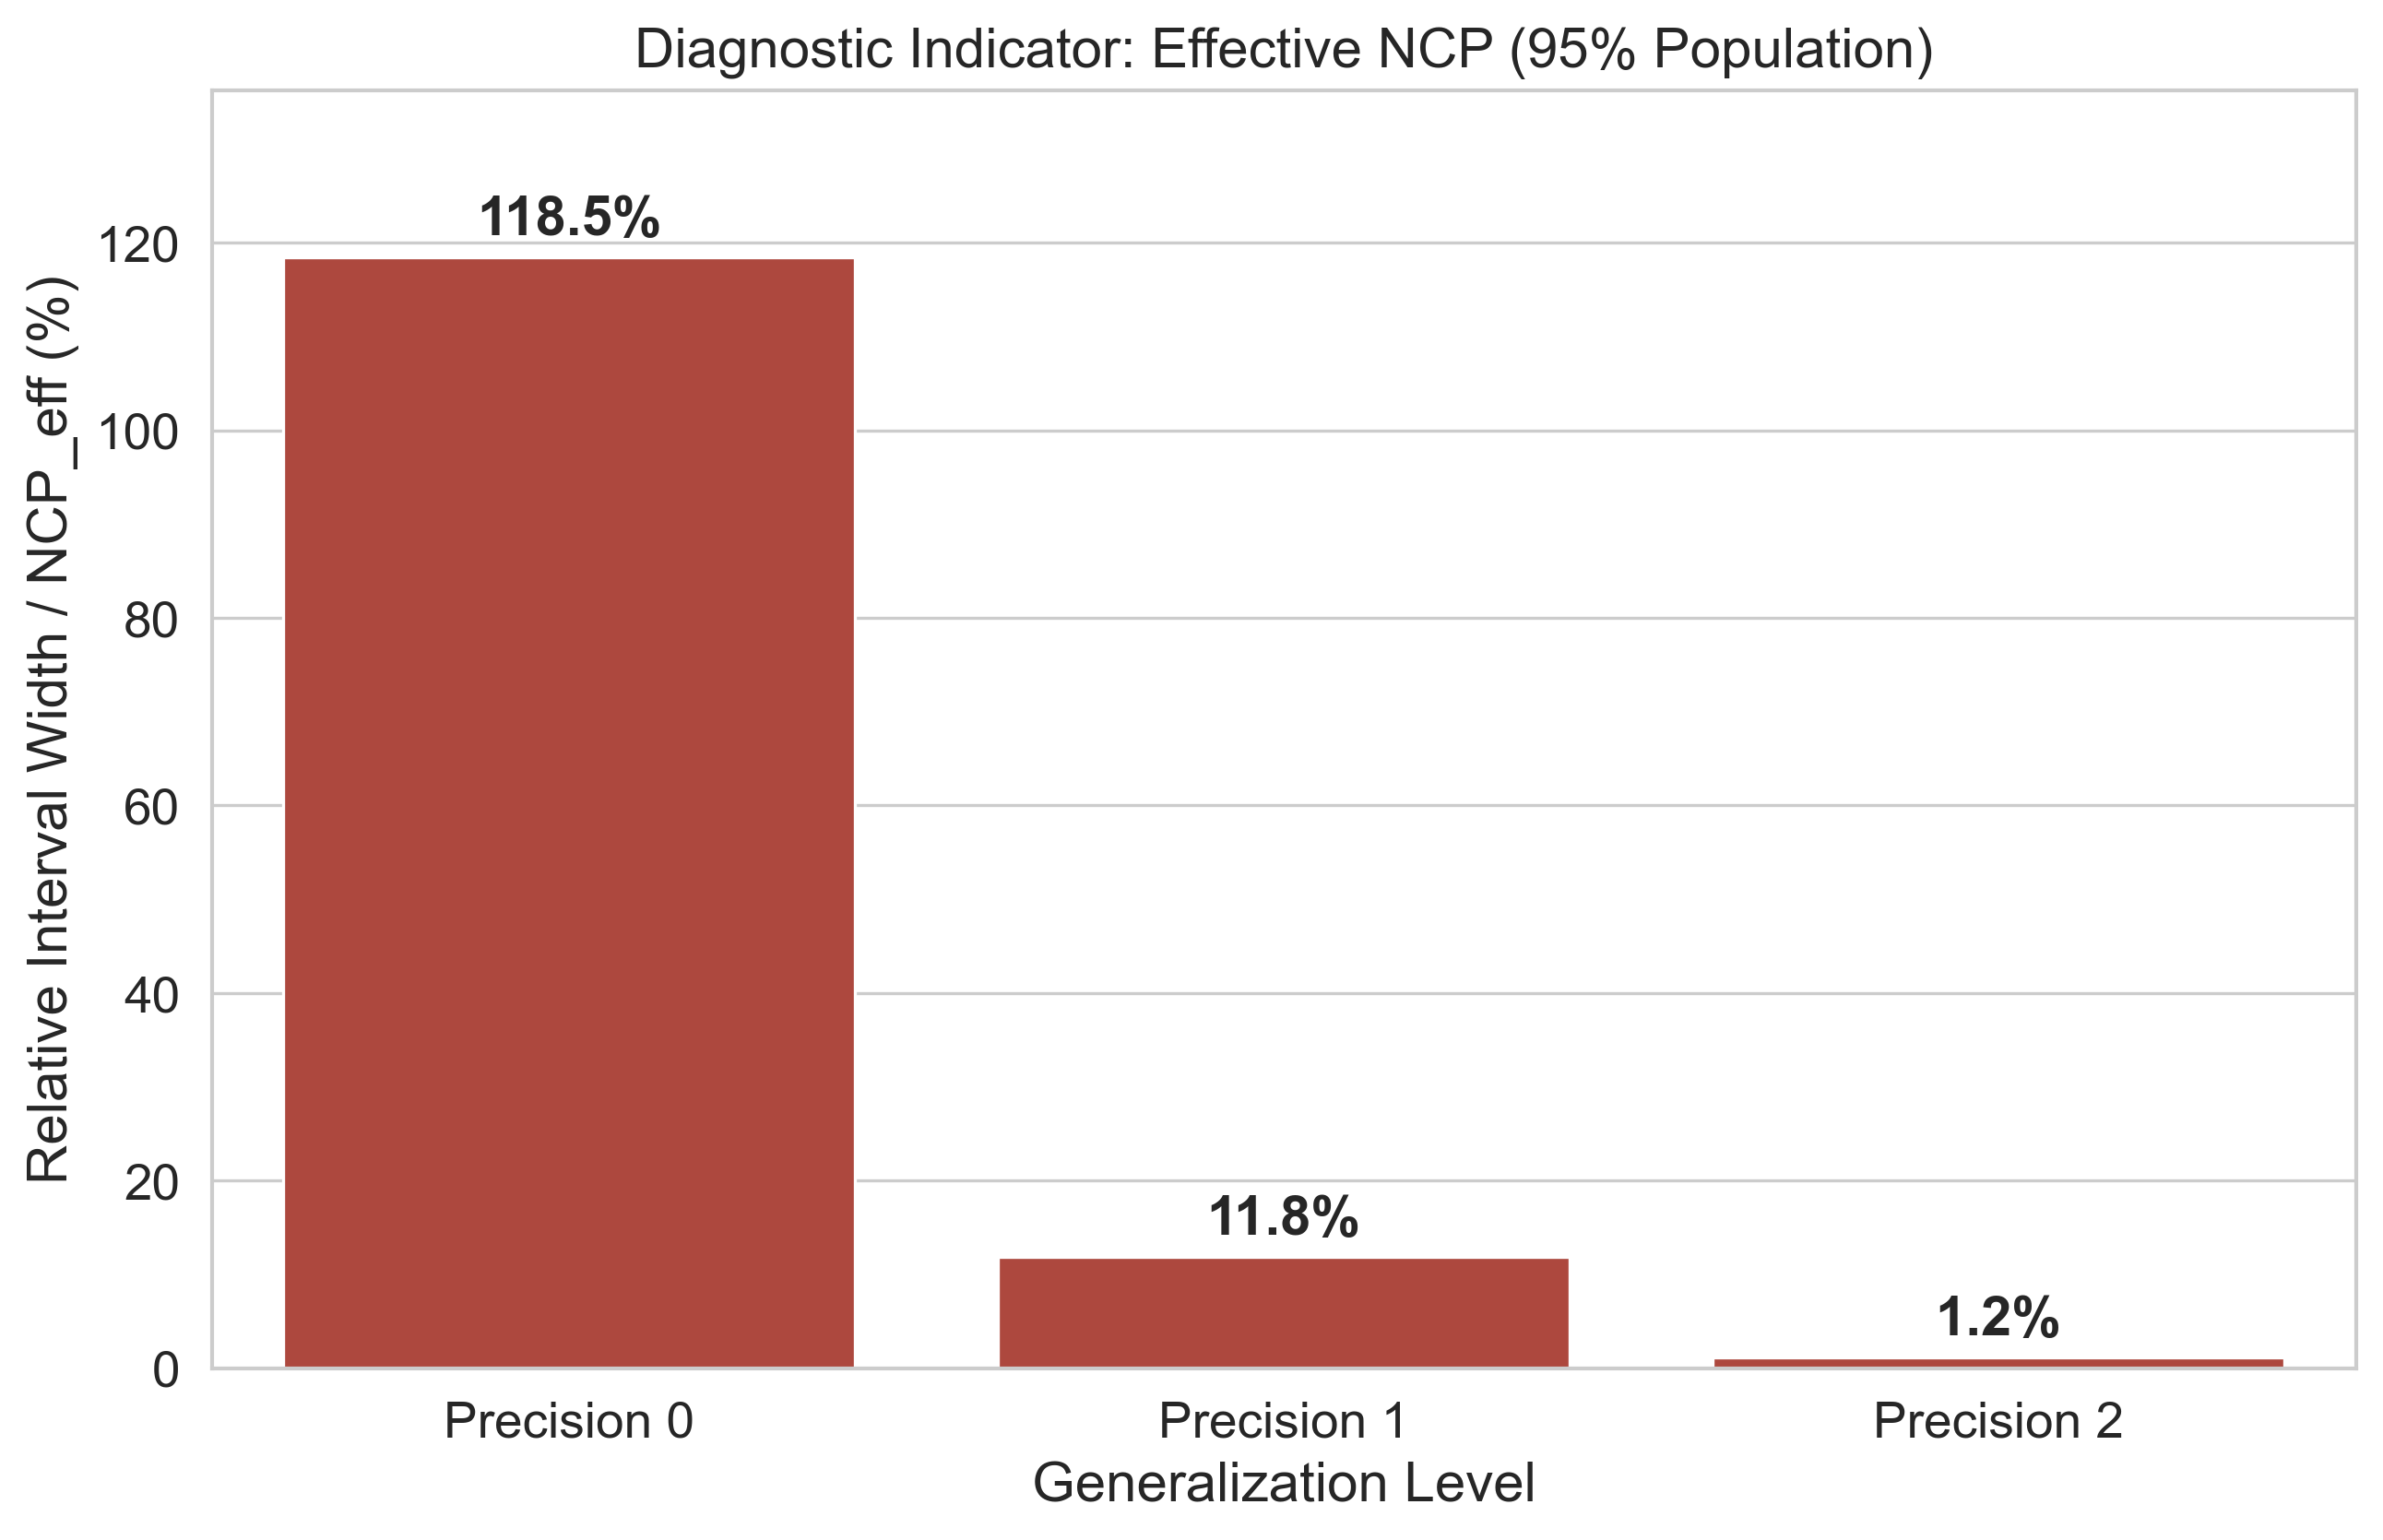
\includegraphics[width=0.75\textwidth]{figures/results_ncp_eff.png}
\caption{Comparison of Standard and Effective NCP. The Effective NCP reveals the true damage to utility for the typical user population.}
\label{fig:encp_comparison}
\end{figure}

The contrast in Figure \ref{fig:encp_comparison} illustrates a significant divergence between the two metrics. While the $\text{NCP}_{\text{std}}$ for Precision 0 is recorded at 10.8\%, the $\text{NCP}_{\text{eff}}$ reaches \textbf{118.5\%}. As defined in the methodology, this value occurs because the rounding interval (1.0 kWh) is numerically larger than the entire consumption span of the 95\% population subset, which covers the interval [0, 0.844 kWh]. In comparison, Precision 1 and Precision 2 yield $\text{NCP}_{\text{eff}}$ values of 11.8\% and 1.2\% respectively, indicating a much closer alignment between the generalization interval and the actual data variance.


% \clearpage


\section{Impact of Temporal Aggregation (Edge)}

The third experimental scenario evaluates the reduction of temporal resolution at the Edge Layer to optimize network performance. Unlike Data Generalization, which modifies numerical values to facilitate grouping, Temporal Aggregation reduces the frequency of data transmission by representing multiple 30-minute intervals with a single arithmetic mean.

Figure \ref{fig:results_agg_bw} illustrates the Bandwidth Savings achieved across the three tested window sizes ($W \in \{1\,\text{h}, 2\,\text{h}, 4\,\text{h}\}$).

\begin{figure}[H]
\centering
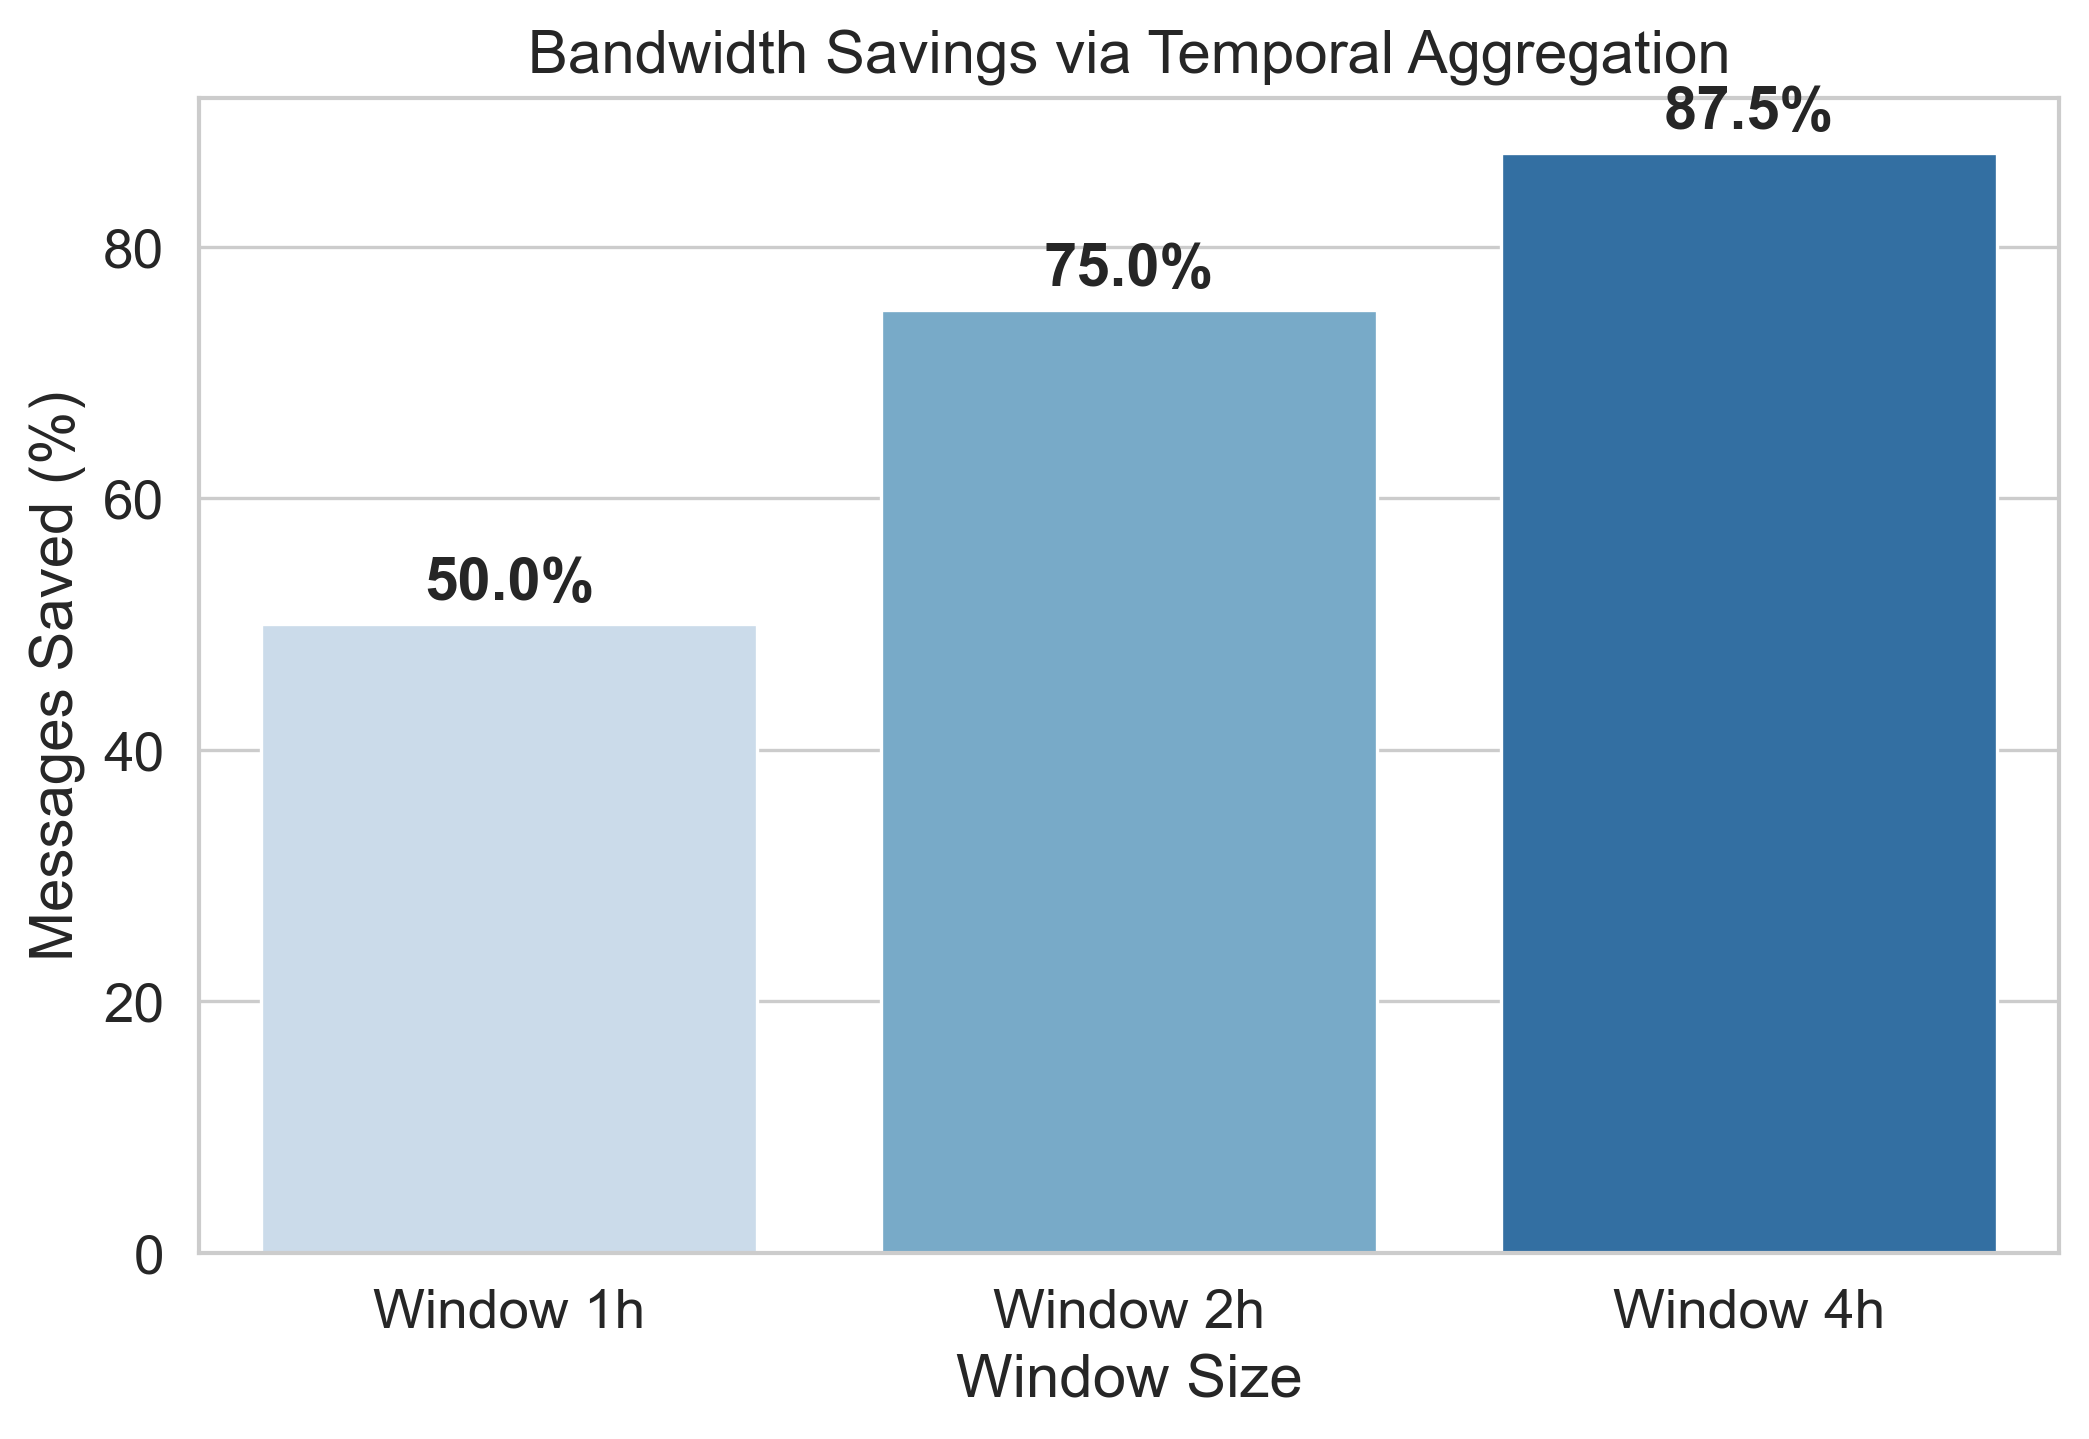
\includegraphics[width=0.75\textwidth]{figures/results_aggregation_bandwidth.png}
\caption{Bandwidth Savings achieved through non-overlapping (tumbling) time windows joining $n$ timestamps. Savings increase with the window size, following a $1-1/n$ relationship.}
\label{fig:results_agg_bw}
\end{figure}


The results confirm that bandwidth savings follow a deterministic relationship ($1-1/n$), where $n$ represents the number of original 30-minute timestamps consolidated into each window. For instance, the 2h window joins $n=4$ intervals, resulting in the theoretical $1 - 1/4 = 75\%$ savings observed in the data.

\begin{itemize}
    \item \textbf{Window 1h (n=2):} Results in a 50.0\% reduction in transmitted tuples, as two 30-minute readings are consolidated into one.
    \item \textbf{Window 2h (n=4):} Achieves 75.0\% savings, significantly reducing the communication overhead for the Edge nodes.
    \item \textbf{Window 4h (n=8)}: Provides the highest performance gain of 87.5\% among the tested configurations, representing an 8-to-1 reduction in data volume.
\end{itemize}

These results show that temporal aggregation enables a predictable reduction in data volume, reaching 87.5\% for the 4h window, while the corresponding Publication Ratio follows the 30-minute baseline trend with minimal deviation.

To assess the impact of these performance gains on data utility, Figure \ref{fig:results_agg_privacy} compares the global publication ratio of the aggregated windows against the 30-minute baseline.

\begin{figure}[H]
\centering
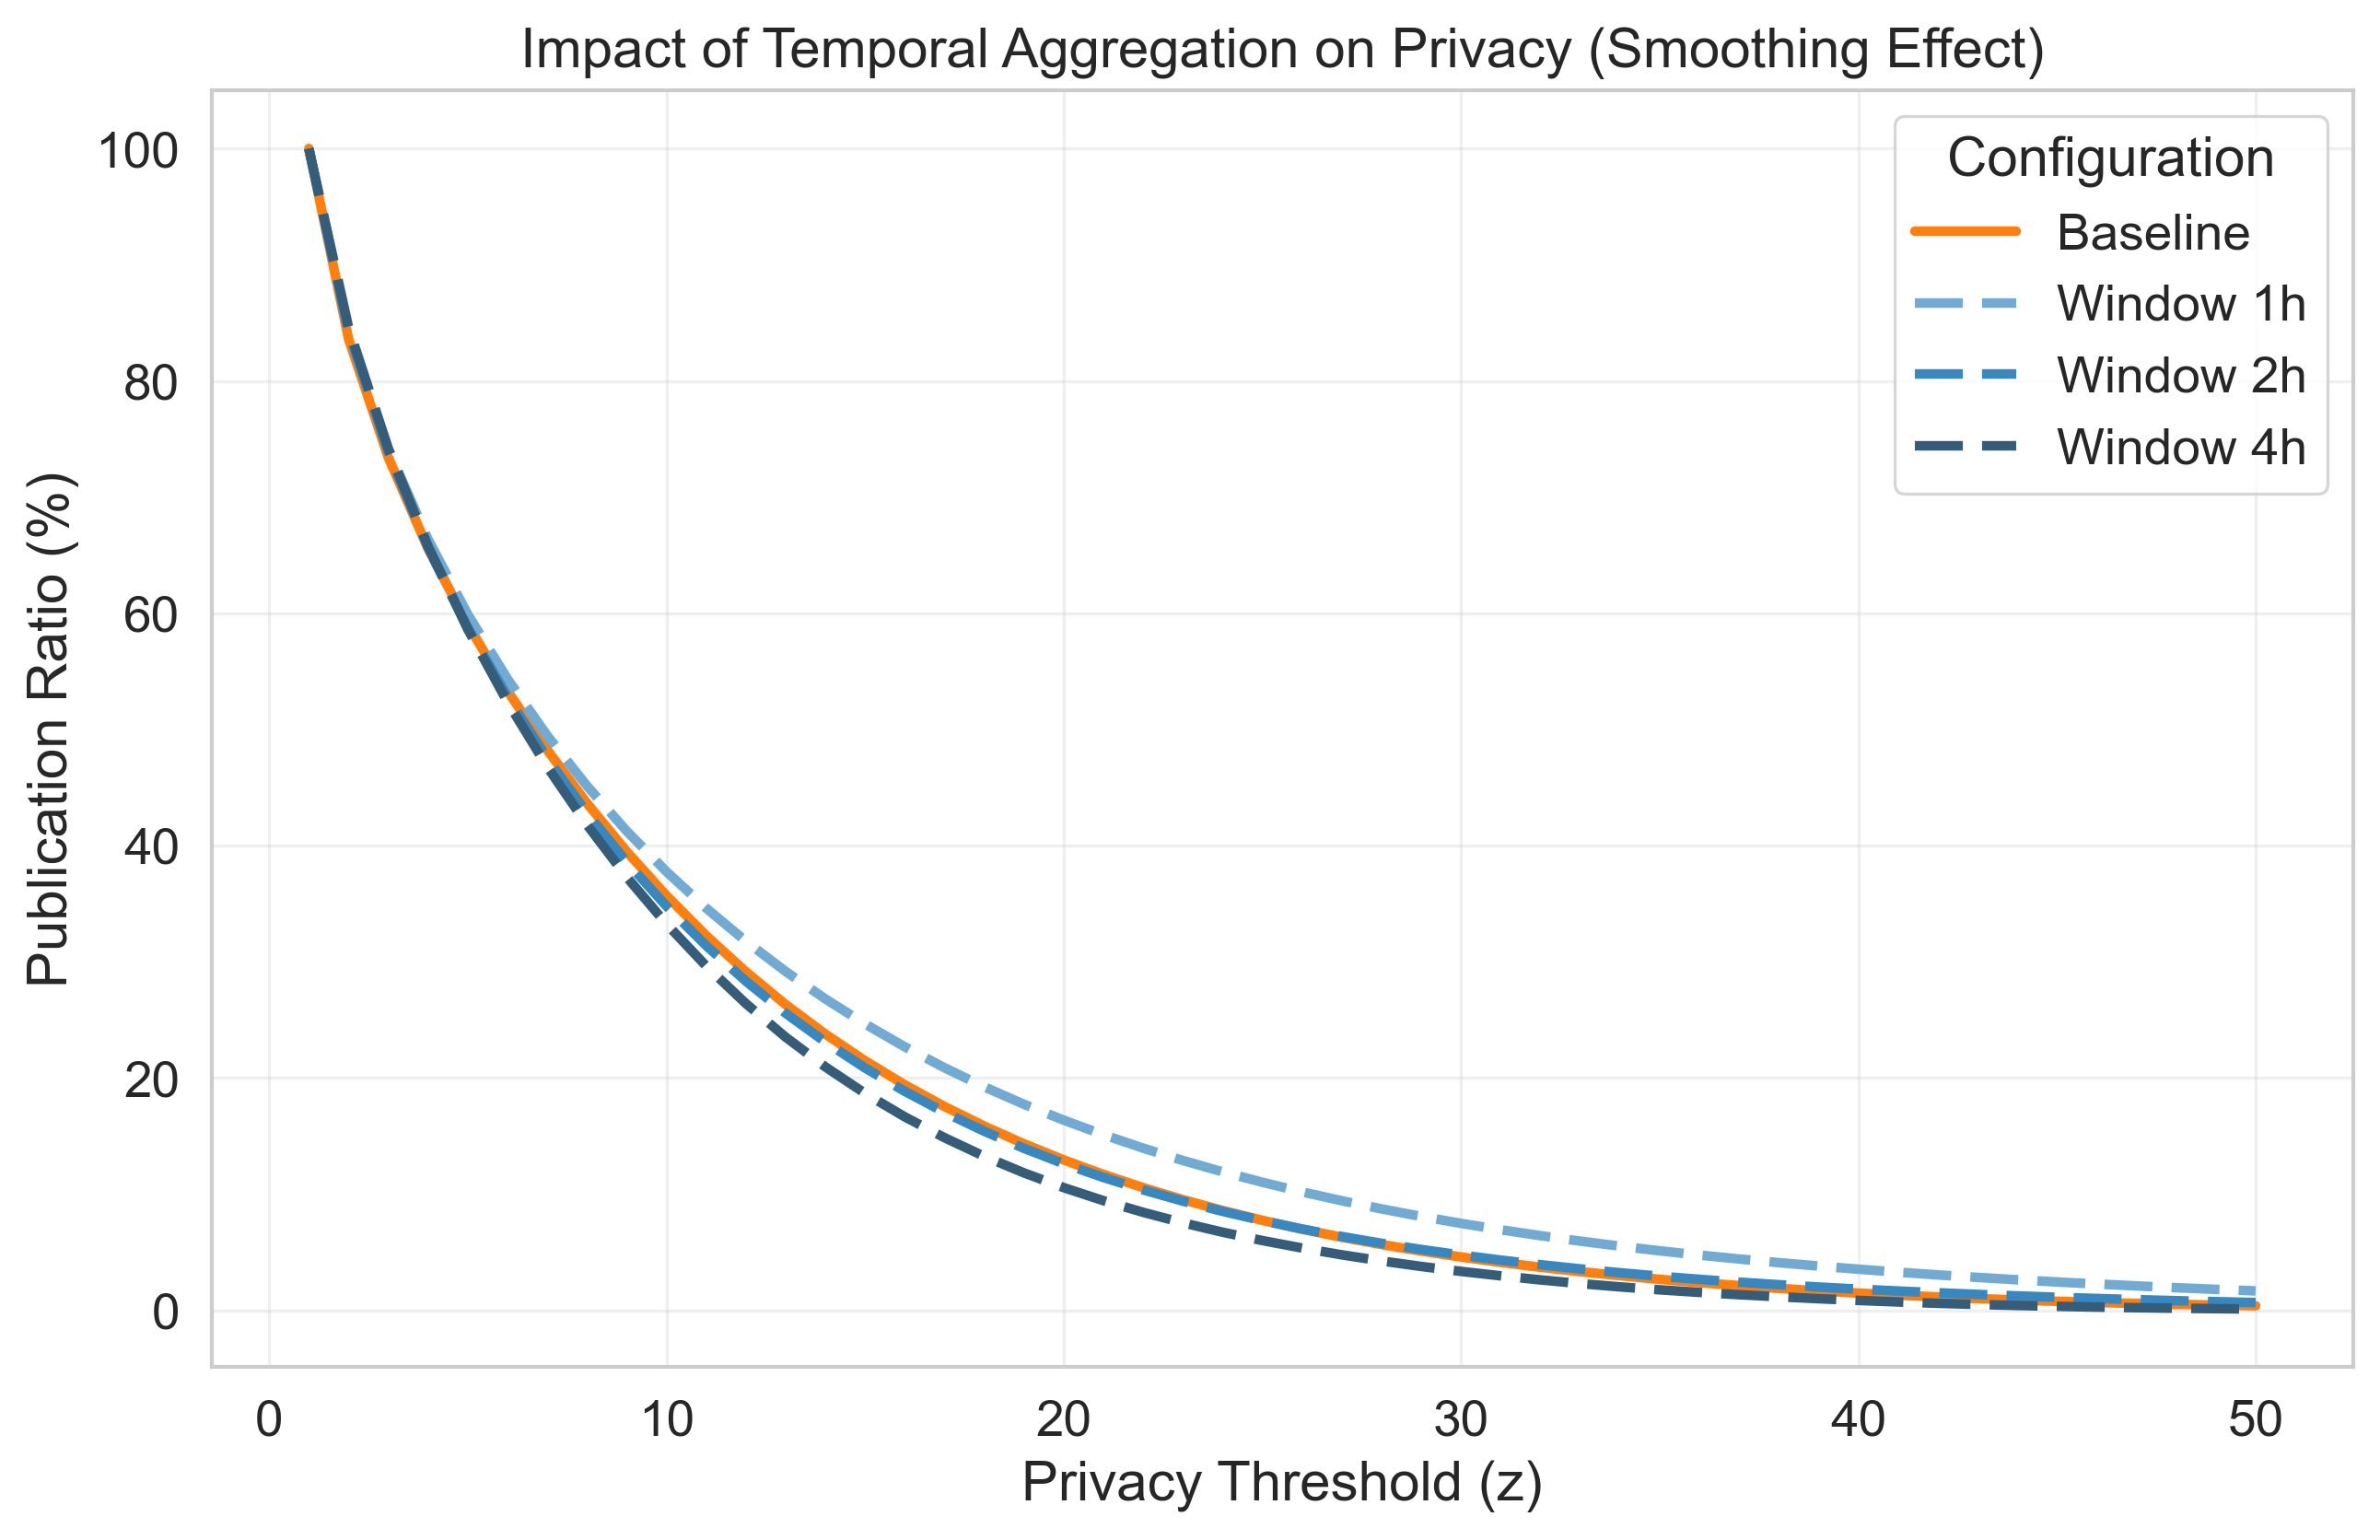
\includegraphics[width=0.85\textwidth]{figures/results_aggregation_privacy.png}
\caption{Comparison of Publication Ratio: Baseline vs. Aggregated Windows. Aggregation results maintain near-total parity with the baseline across all tested thresholds.}
\label{fig:results_agg_privacy}
\end{figure}




The experimental data illustrated in Figure \ref{fig:results_agg_privacy} shows that the publication ratios for the aggregated windows follow a trajectory nearly identical to the 30-minute baseline. Across the tested range of $z$, the availability for the \textbf{Window 1h} and \textbf{Window 2h} scenarios remains marginally higher than the baseline. Specifically, at the highest tested threshold of $z=50$, the 1h window reports a publication ratio of 1.68\%, compared to the 0.40\% observed in the baseline.

The \textbf{Window 4h} scenario results in an 87.5\% reduction in total record count. At $z=50$, its publication ratio (0.11\%) remains within a 0.3 percentage point absolute range of the baseline. Across all tested configurations, the difference in data availability between the 30-minute raw data and the aggregated windows does not exceed a 1.3 percentage point absolute margin at $z=50$.


\section{Impact of Local Prefiltering}
\label{sec:localprefiltering}

The final scenario evaluates a distributed architecture where the privacy-preserving workload is shared between the Fog gateways and the Central Entity. This hybrid approach combines data generalization at the Edge with a Snapshot $z$-anonymity check at the Fog Layer. For this configuration, a fixed precision of \textbf{$p=2$ decimal places} was chosen. As justified in the methodology (Section~\ref{sec:scenarios}), this choice was based on a preliminary analysis which revealed that raw data ($p=3$) is too unique within a small 100-user neighborhood to satisfy a local $z$-threshold, leading to near-total suppression at the gateway. Generalizing to two decimal places provides the minimum data density required to make localized prefiltering a viable architectural strategy.


% This hybrid approach combines data generalization ($p=2$) at the Edge with a snapshot $z$-anonymity check at the Fog level.


Figure \ref{fig:results_prefilter_ratio} illustrates the global publication ratio for three local thresholds ($z_{\text{local}} \in \{2, 5, 10\}$) compared to the raw 30-minute baseline. To establish an upper bound for data utility, a standalone $p=2$ generalization curve (Edge Only) is included as a reference.

\begin{figure}[H]
\centering
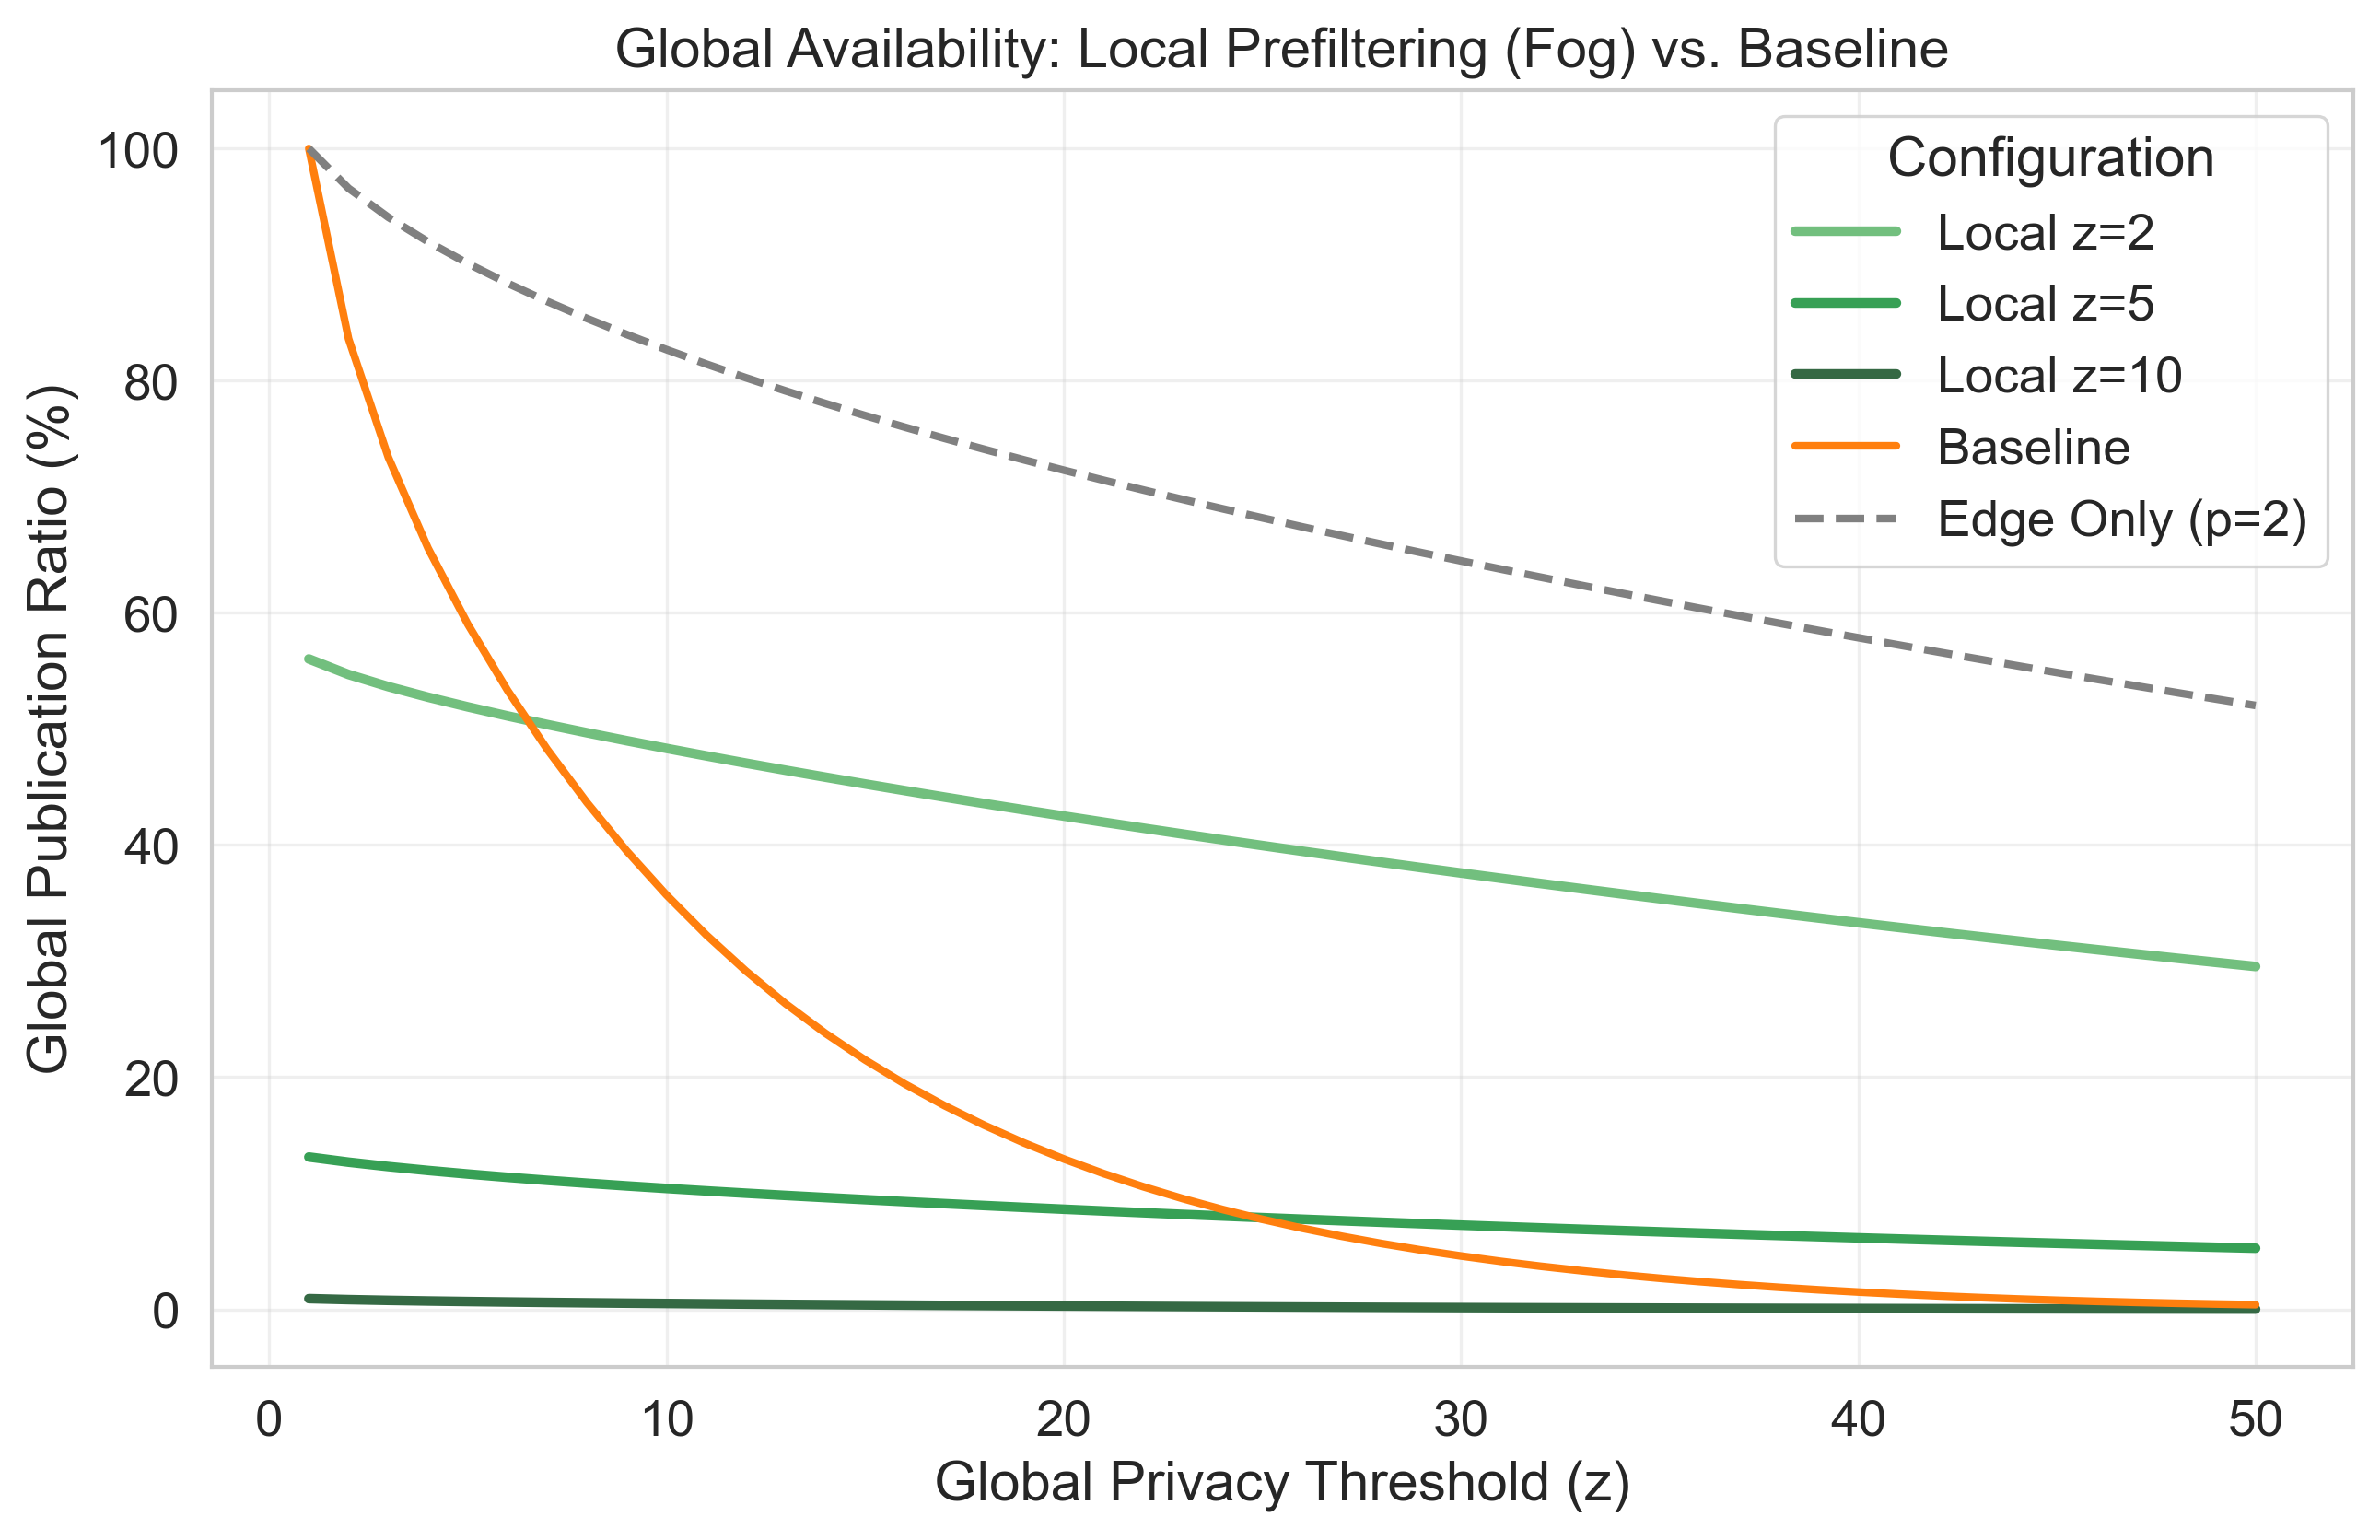
\includegraphics[width=0.85\textwidth]{figures/results_prefiltering_ratio.png}
\caption{Global Publication Ratio after Local Prefiltering. Availability is heavily dependent on the local suppression threshold.}
\label{fig:results_prefilter_ratio}
\end{figure}


The data reveals two distinct behaviors driven by the interaction between precision reduction and local filtering:

\begin{itemize}
    \item \textbf{Initial Suppression:} At $z=1$, the \textbf{Local $z=2$} scenario publishes 56.03\% of data, representing a 43.97 percentage point absolute drop compared to the 100\% availability of the standalone Edge Only $p=2$ reference. Because both scenarios use identical Edge rounding, this initial gap represents the suppression overhead introduced by the Fog Layer. Data that is frequent enough globally is suppressed because it fails to meet the threshold within its specific local neighborhood. The \textbf{Local $z=5$} and \textbf{Local $z=10$} scenarios experience even steeper initial suppression, starting at 13.12\% and 0.92\% respectively.
    \item \textbf{Decline Rate:} Despite the lower starting points, the prefiltering curves follow a slow-decay trajectory nearly parallel to the standalone Edge Only $p=2$ reference, rather than the sharp drop of the raw baseline. At $z=50$, the raw baseline falls to 0.4\%, whereas the \textbf{Local $z=2$} scenario maintains 29.53\% availability (compared to 52.02\% for the standalone $p=2$ case). The absolute gap between these two curves narrows as $z$ increases, shifting from a 43.98 percentage point difference at $z=1$ to 22.49 percentage points at $z=50$.
\end{itemize} 

Figure \ref{fig:results_prefilter_offloading} illustrates the "Success Rate at Cloud", which measures the percentage of tuples that were not suppressed by the local Fog Layer filter and subsequently satisfied the global $z$ requirement.

\begin{figure}[H]
\centering
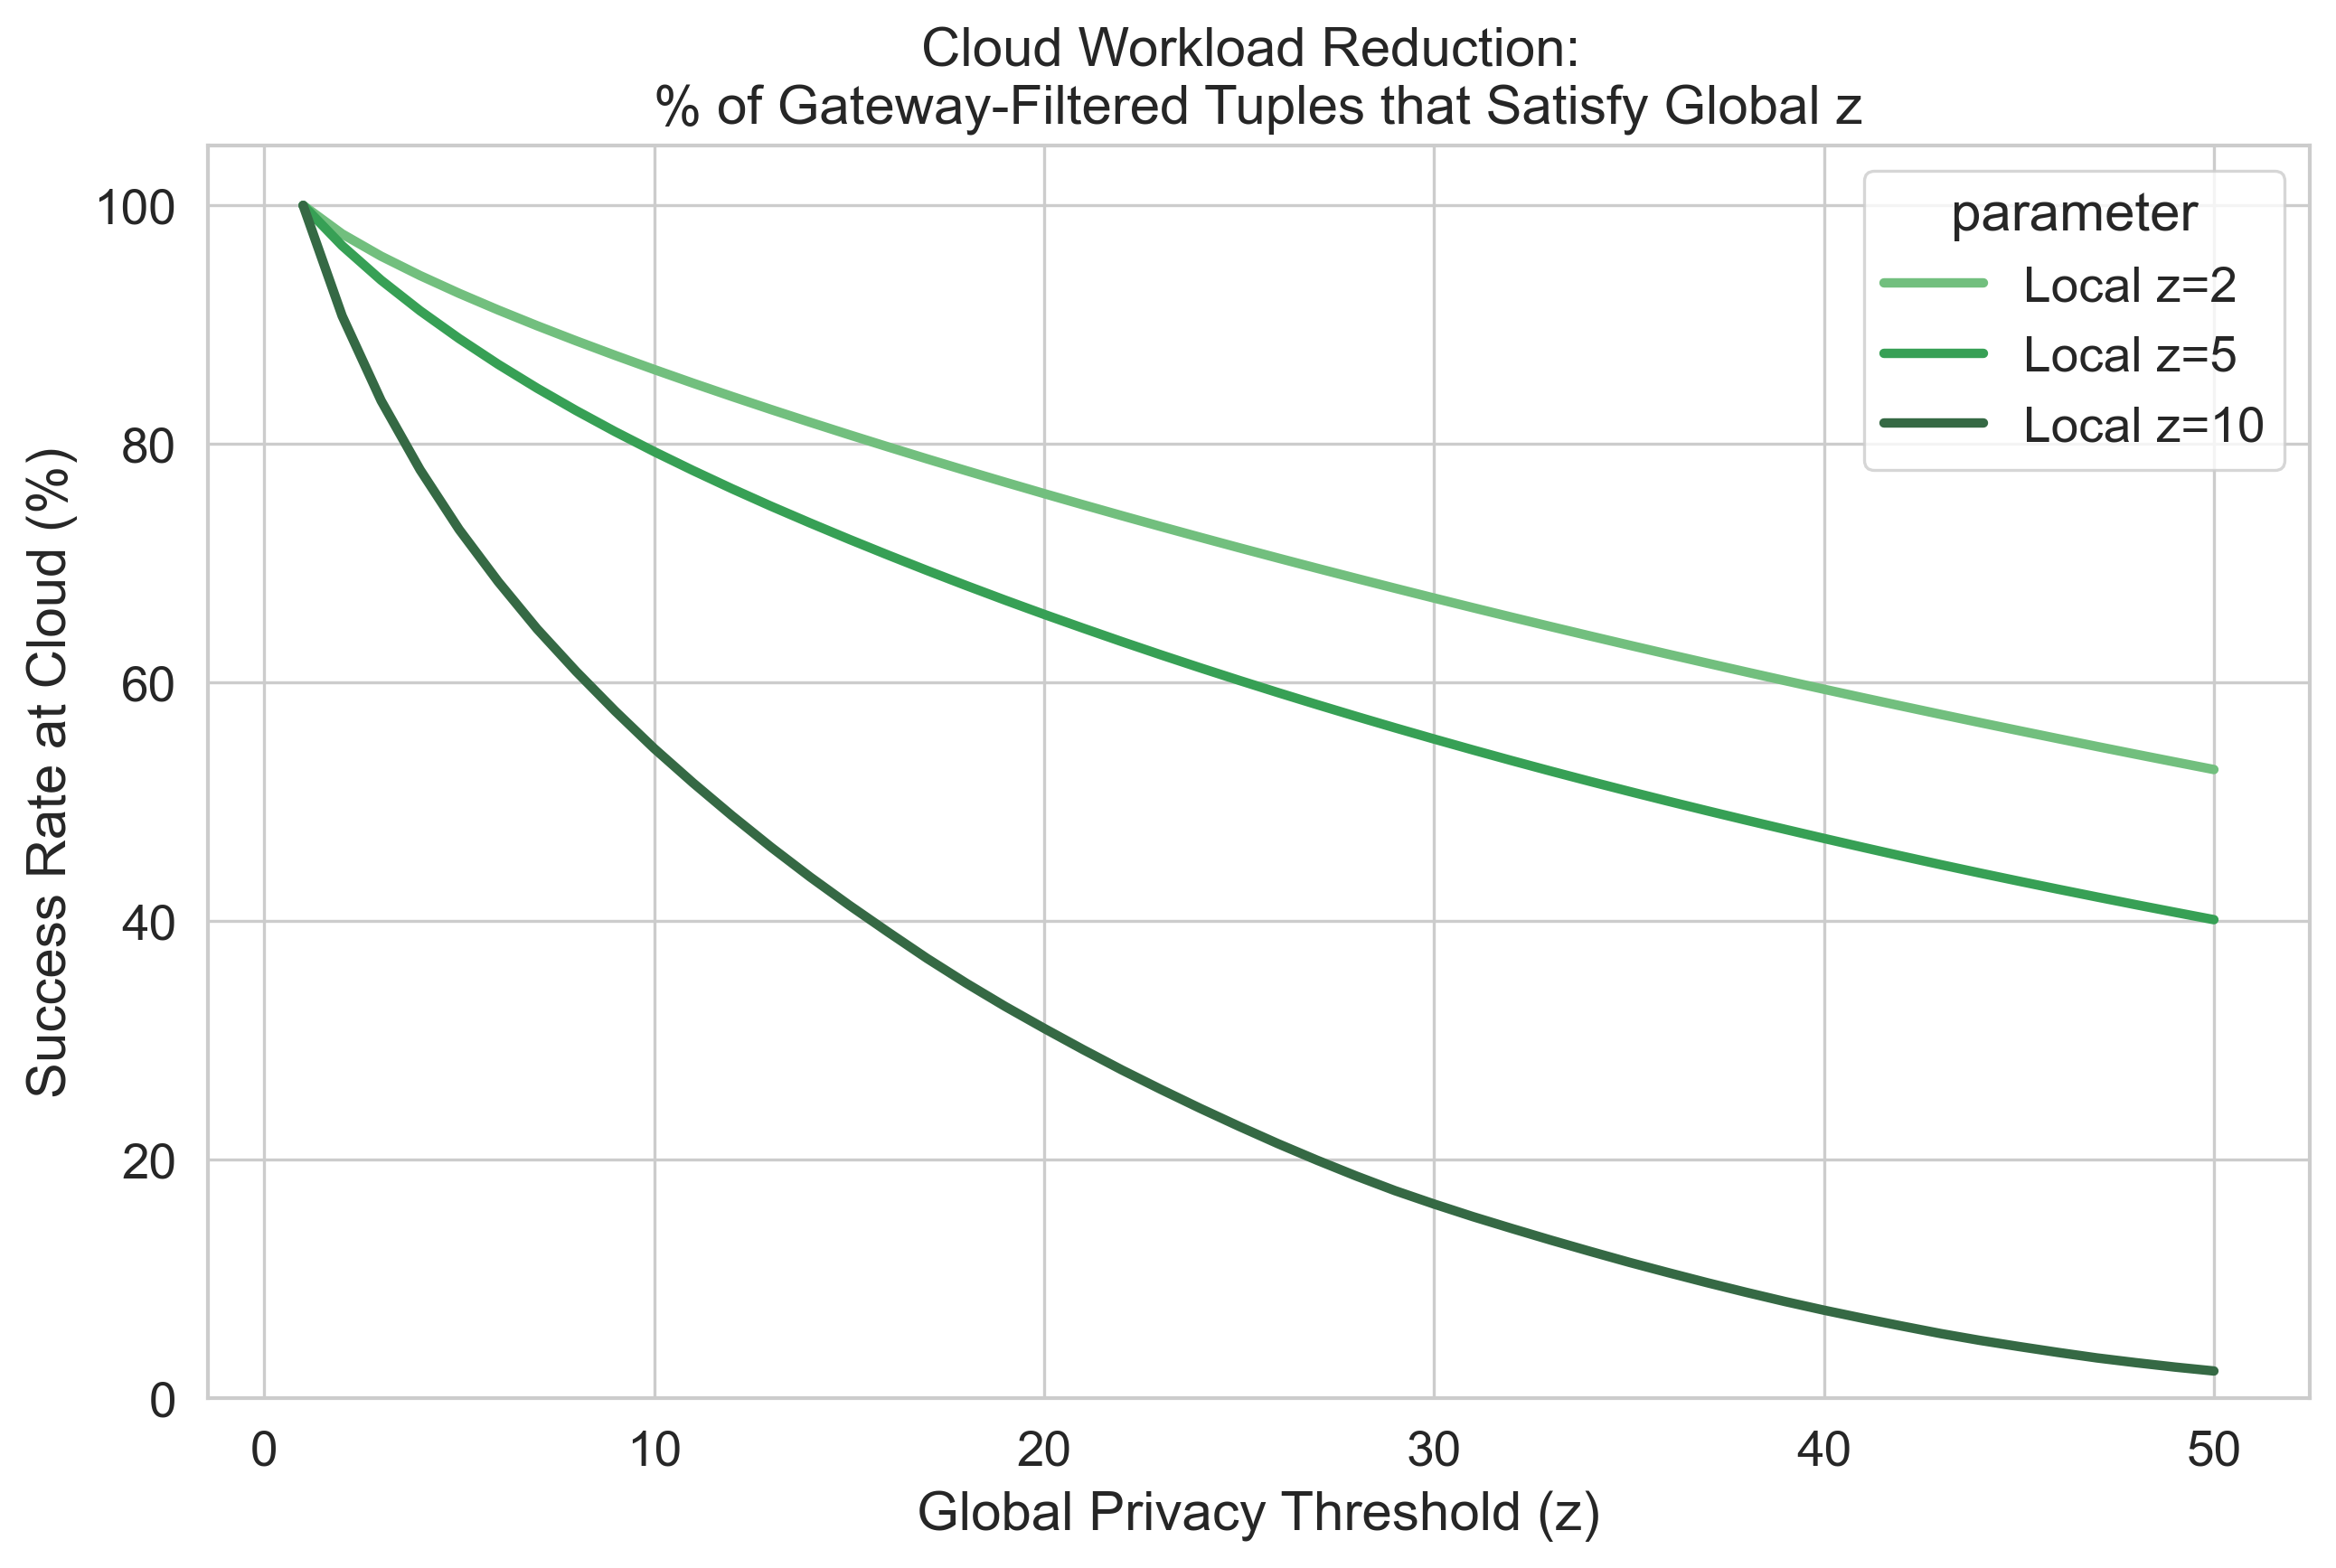
\includegraphics[width=0.85\textwidth]{figures/results_prefiltering_offloading.png}
\caption{Cloud Workload Reduction: Percentage of Gateway-Filtered tuples that satisfy the Global z threshold.}
\label{fig:results_prefilter_offloading}
\end{figure}




The data shows that while all scenarios begin with a 100\% success rate at $z=1$, the proportion of Fog-approved tuples that pass the Cloud-level check decreases as the global threshold $z$ increases. This decline is most pronounced in the \textbf{Local $z=10$} scenario, where the success rate drops to approximately 2.29\% at $z=50$. This trend indicates a cumulative suppression effect: because the gateways subtract $(z_{\text{local}} - 1)$ from the local counts before forwarding, the Central Entity receives a significantly reduced data stream. Consequently, this depletion causes the success rate to drop even when the global threshold matches the local filter (e.g., when both are set to $z=5$). Furthermore, this mechanism explains why the success rate falls much faster for $z_{\text{local}}=10$ and $z_{\text{local}}=5$ compared to $z_{\text{local}}=2$. A higher local threshold filters out a significantly larger portion of tuples at the Fog Layer, resulting in a much smaller surplus being forwarded. Consequently, to survive the final global check, multiple gateways must simultaneously report a surplus for the exact same value, which becomes increasingly improbable when the forwarded volumes are already severely depleted by strict local filters.


In addition to the impacts on data utility, this scenario results in a reduction of message volume between the Fog and Cloud Layers. By suppressing unique outliers before they traverse the core network, the architecture generates significant bandwidth savings. Because a global threshold of $z=1$ effectively disables suppression at the Central Entity (as any count $\geq 1$ is published), the global publication ratio at this point strictly reflects the data that passed the local gateways. Therefore, the data "missing" at $z=1$ in Figure \ref{fig:results_prefilter_ratio} represents the exact percentage of tuples blocked at the Fog Layer, translating directly to the following bandwidth savings:

\begin{itemize}
    \item \textbf{Local $z=2$:} Achieves a 43.97\% reduction in message volume.
    \item \textbf{Local $z=5$:} Achieves an 86.88\% reduction, effectively removing the vast majority of unique consumption spikes from the stream.
    \item \textbf{Local $z=10$:} Suppresses 99.08\% of all generated data at the gateway level.
\end{itemize}

The data shows a consistent inverse relationship between bandwidth savings at the Fog Layer and subsequent data availability at the Central Entity. As the local threshold increases from $z_{\text{local}}=2$ to $z_{\text{local}}=10$, the resulting bandwidth savings increase from 43.97\% to 99.08\%, while the initial global publication ratio ($z=1$) decreases from 56.03\% to 0.92\%. Across the evaluated configurations, the local threshold acts as an upper bound for the maximum achievable data utility at the Central Entity.